\documentclass[12pt,a4paper]{report}
\usepackage[utf8]{inputenc}
\usepackage[T1]{fontenc}
\usepackage{babel}
\usepackage{graphicx}
\usepackage{float}
\usepackage[hidelinks]{hyperref}
\usepackage{geometry}
\geometry{margin=1in}
\usepackage{setspace}
\setstretch{1.3}
\setlength{\parskip}{0.4em}
\usepackage{amsmath}
\usepackage{amssymb} % for \checkmark
\usepackage{textcomp} % for \texttimes
\usepackage{array}
\usepackage{longtable}
\usepackage{booktabs}
\usepackage{xcolor}
\usepackage{enumitem}
\usepackage{fancyhdr}
\usepackage[most]{tcolorbox}

% ── Default page style: footer only (line + page number right) ─────────────
\pagestyle{fancy}
\fancyhf{}
\fancyfoot[R]{\thepage}
\renewcommand{\footrulewidth}{0.4pt}
\renewcommand{\headrulewidth}{0pt}
% Ensure subsubsections are numbered and added to the Table of Contents
\setcounter{secnumdepth}{3}
\setcounter{tocdepth}{3}
% ── Chapter page style: banner in header + footer ────────────────────────
\fancypagestyle{chapterone}{%
    \fancyhf{}
    % Header: "Chapter 1" italic then full rule
    \fancyhead[L]{%
        \textit{Chapter 1}\\[-4pt]
        \rule{\textwidth}{0.4pt}%
    }
    \renewcommand{\headrulewidth}{0pt}
    % Footer: rule + page number right
    \fancyfoot[R]{\thepage}
    \renewcommand{\footrulewidth}{0.4pt}
}
\fancypagestyle{chaptertwo}{%
    \fancyhf{}
    \fancyhead[L]{%
        \textit{Chapter 2}\\[-4pt]
        \rule{\textwidth}{0.4pt}%
    }
    \renewcommand{\headrulewidth}{0pt}
    \fancyfoot[R]{\thepage}
    \renewcommand{\footrulewidth}{0.4pt}
}
\fancypagestyle{chapterthree}{%
    \fancyhf{}
    \fancyhead[L]{%
        \textit{Chapter 3}\\[-4pt]
        \rule{\textwidth}{0.4pt}%
    }
    \renewcommand{\headrulewidth}{0pt}
    \fancyfoot[R]{\thepage}
    \renewcommand{\footrulewidth}{0.4pt}
}
\fancypagestyle{chapterfour}{%
    \fancyhf{}
    \fancyhead[L]{%
        \textit{Chapter 4}\\[-4pt]
        \rule{\textwidth}{0.4pt}%
    }
    \renewcommand{\headrulewidth}{0pt}
    \fancyfoot[R]{\thepage}
    \renewcommand{\footrulewidth}{0.4pt}
}
% Add these packages for Arabic support
\usepackage{polyglossia}
\setmainlanguage{french} % Assuming French is your main document language
\setotherlanguage{arabic}

% Amiri is a great, standard Arabic font pre-installed on Overleaf
\newfontfamily\arabicfont[Script=Arabic]{Amiri}
\begin{document}

% ==================== TITLE PAGE ====================
\begin{titlepage}
    \thispagestyle{empty}
    \centering

    \begin{minipage}[c]{0.40\linewidth}
        \centering
        
\includegraphics[height=2.0cm]{enicar.jpg}
    \end{minipage}
    \hfill
    \begin{minipage}[c]{0.50\linewidth}
        \raggedleft
        {\small \textbf{National School of Engineers of Carthage}\\[2pt]
        \textsc{ENICarthage --- University of Carthage}}
    \end{minipage}

    \vspace{0.2cm}
    \noindent\rule{\linewidth}{0.4pt}
    \vspace{0.1cm}

    {\normalsize Ministry of Higher Education and Scientific Research\par}

    \vspace{0.2cm}

    {\normalsize \textit{Specialty :}\par}
    {\normalsize Computer Science\par}

    \vspace{0.3cm}

    {\LARGE \textbf{End-of-Studies Project Report}\par}

    \vspace{0.1cm}

    \begin{flushleft}
    {\large \textit{Theme :}\par}
    \end{flushleft}

    {\Large \textbf{\guillemotleft~AI-Powered Automated Penetration Testing~\guillemotright}\par}

    \vspace{1cm}

    {\normalsize \textit{Performed by :}\par}
    \vspace{0.2cm}
    {\large \textbf{Hosni Raissi}\par}

    \vspace{0.3cm}

    {\normalsize \textit{Professional Supervisor:} Mr. Walid Bensaïd\par}
    \vspace{0.1cm}
    {\normalsize \textit{Academic Supervisor:} Mr. Houcem Hermassi\par}

    \vspace{0.5cm}

    {\normalsize \textit{Work proposed and carried out in collaboration with}\par}
    \vspace{0.3cm}
    
\includegraphics[width=0.28\linewidth]{talan1.png}

    \vspace{0.1cm}

    {\normalsize Academic year : 2025--2026\par}
    \vspace{0.1cm}
    \vfill

    \noindent
    \colorbox{gray!15}{%
        \begin{minipage}{\dimexpr\linewidth}
            \centering
            \vspace{0.25cm}
            {\small National School of Engineers of Carthage\\
            \textbf{ENICarthage}\\
            \textit{45 Avenue des Entrepreneurs, 2035 Charguia II, Tunis-Carthage, Tunisia}\\
            Tel. (+216) 71 941 579 / (+216) 71 940 699 \textendash\ Website: www.enicarthage.rnu.tn}
            \vspace{0.25cm}
        \end{minipage}
    }

\end{titlepage}

% ==================== SIGNATURES ====================
\newpage
\thispagestyle{empty}

{\fontsize{24}{28}\selectfont \textbf{Signatures}}\par

\vspace{0.8cm}

\begin{tcolorbox}[
    enhanced,
    colback=white,
    colframe=black!70,
    boxrule=0.9pt,
    arc=4mm,
    width=\textwidth,
    left=12mm,
    right=12mm,
    top=11mm,
    bottom=11mm
]
I authorize the student to submit the internship report for evaluation.

\vspace{1.1cm}

\centering
Professional Supervisor, \textbf{Mr.\ Walid Bensa\"{i}d}

\vspace{1.6cm}

\begin{flushright}
\textbf{Signature and Stamp}
\end{flushright}
\end{tcolorbox}

\vspace{1.1cm}

\begin{tcolorbox}[
    enhanced,
    colback=white,
    colframe=black!70,
    boxrule=0.9pt,
    arc=4mm,
    width=\textwidth,
    left=12mm,
    right=12mm,
    top=11mm,
    bottom=11mm
]
I authorize the student to submit the internship report for evaluation.

\vspace{1.1cm}

\centering
Academic Supervisor, \textbf{Mr.\ Houcem Hermassi}

\vspace{1.6cm}

\begin{flushright}
\textbf{Signature}
\end{flushright}
\end{tcolorbox}

% ==================== ABSTRACT ====================
\newpage
\thispagestyle{fancy}
\section*{Abstract}

This work is part of the end-of-studies project of the National School of Engineers of Carthage (ENICarthage), aiming to obtain the national engineering degree in Computer Science. It was conducted during a four-month internship at Talan.

Faced with rapidly expanding attack surfaces and a global shortage of cybersecurity professionals, organizations must innovate their offensive security strategies. In response to this challenge, an open-source, AI-powered automated penetration testing platform named PentaForge has been developed and detailed in this report. This solution automates the complete penetration testing lifecycle—from reconnaissance to reporting—primarily relying on a secure, multi-agent architecture and a robust data sanitization layer to ensure confidentiality.

\vspace{0.4cm}
\noindent \textbf{Keywords:} Automated penetration testing, Artificial intelligence,
Multi-agent system, RAG, LLM, CVSS, Cybersecurity, PentaForge.

% ==================== RÉSUMÉ ====================
\section*{R\'{e}sum\'{e}}

Ce travail s'inscrit dans le cadre du projet de fin d'\'{e}tudes de l'\'{E}cole Nationale
d'Ing\'{e}nieurs de Carthage (ENICarthage), en vue de l'obtention du dipl\^{o}me national
d'ing\'{e}nieur en Informatique. Il a \'{e}t\'{e} r\'{e}alis\'{e} lors d'un stage de quatre mois au sein de Talan.

Face à l'expansion rapide des surfaces d'attaque et à la pénurie mondiale de professionnels qualifiés en cybersécurité, les organisations doivent innover dans leurs stratégies de sécurité offensive. En réponse à ce défi, une plateforme open-source de tests d'intrusion automatisés pilotée par l'intelligence artificielle, nommée PentaForge, a été développée et détaillée dans ce rapport. Cette solution automatise l'intégralité du cycle de pentest — de la reconnaissance jusqu'à la rédaction de rapports — en s'appuyant principalement sur une architecture multi-agents sécurisée et une couche de sanitisation systématique des données pour en garantir la confidentialité.

\vspace{0.4cm}
\noindent \textbf{Mots-cl\'{e}s :} Tests d'intrusion automatis\'{e}s, Intelligence artificielle,
Syst\`{e}me multi-agents, RAG, LLM, CVSS, Cybers\'{e}curit\'{e}, PentaForge.

% ==================== DEDICATIONS ====================
\newpage
\thispagestyle{fancy}
\section*{Dedications}

\vspace{1.2cm}

To my family, unwavering pillar of my life, this work is dedicated to you.
Your love, support, and faith in me have been the foundation of all my successes.

\vspace{1cm}

To my parents, whose wisdom, dedication, and sacrifices have lit every step of my path.
Your unconditional love gave me the strength and determination to overcome every obstacle.

\vspace{1cm}

To my two brothers and my sister, companions at all times, who shared with me
the laughter, the challenges, and the aspirations. Your camaraderie and support
enriched every moment of this adventure.

\vspace{1cm}

To my close friends, who have always been there. Your friendship, encouragement,
and advice played a crucial role in my journey. Your presence and feedback
often guided my choices when it mattered most.

\vspace{1.4cm}

\begin{flushright}
\itshape
To all of you, I dedicate this work as a sign of my deep gratitude\\
and eternal affection.
\end{flushright}

% ==================== ACKNOWLEDGMENTS ====================
\newpage
\thispagestyle{fancy}
\section*{Acknowledgments}

\vspace{1cm}

First and foremost, I wish to express my sincere gratitude to the National School
of Engineers of Carthage (ENICarthage) for the quality of education and the
stimulating academic environment that shaped both my technical and professional path.

\vspace{0.9cm}

I sincerely thank \textbf{Talan} for welcoming me into their team and for providing
me with the opportunity to deepen my knowledge within a demanding professional
environment.

\vspace{0.9cm}

A special thank you to \textbf{Mr.\ Walid Bensaid}, my internship supervisor at Talan,
for his guidance, patience, and invaluable advice throughout this experience.
His support was a constant and decisive source of learning.

\vspace{0.9cm}

I also extend my deepest gratitude to \textbf{Mr.\ Houcem Hermassi} for agreeing
to supervise this work on behalf of ENICarthage. Your advice and recommendations
enlightened my path and were of great help in carrying out this project.

\vspace{0.9cm}

My thanks also go to the \textbf{Talan Cytest team}, whose collaborative spirit,
constructive feedback, and daily commitment were essential to the completion
of this work.

\vspace{0.9cm}

I would like to express my gratitude to the \textbf{members of the jury} for the time
they dedicate to evaluating this work and for their valuable remarks.

\vspace{1.1cm}

\begin{flushright}
\itshape
Finally, I thank all those who, near or far, played a role\\
in my training and in the success of this project.
\end{flushright}

% ==================== TABLE OF CONTENTS ====================
\newpage
\renewcommand{\contentsname}{Table of Contents}
\tableofcontents

% ==================== LIST OF FIGURES ====================
\newpage
\renewcommand{\listfigurename}{List of Figures}
\listoffigures

% ==================== LIST OF TABLES ====================
\newpage
\renewcommand{\listtablename}{List of Tables}
\listoftables

% ==================== ACRONYMS ====================
\newpage
\thispagestyle{fancy}
\section*{Acronyms}
\addcontentsline{toc}{chapter}{Acronyms}

\begin{longtable}{>{\bfseries}p{3.5cm} p{10.5cm}}
\toprule
\textbf{Acronym} & \textbf{Definition} \\
\midrule
\endhead
AI          & Artificial Intelligence \\
API         & Application Programming Interface \\
CISA        & Cybersecurity and Infrastructure Security Agency \\
CISA KEV    & CISA Known Exploited Vulnerabilities \\
CIS         & Center for Internet Security \\
CLI         & Command Line Interface \\
CVE         & Common Vulnerabilities and Exposures \\
CVSS        & Common Vulnerability Scoring System \\
CWE         & Common Weakness Enumeration \\
DAST        & Dynamic Application Security Testing \\
EPSS        & Exploit Prediction Scoring System \\
FP          & False Positive \\
HITL        & Human-in-the-Loop \\
IoC         & Indicator of Compromise \\
IT          & Information Technology \\
JWT         & JSON Web Token \\
LLM         & Large Language Model \\
MITRE ATT\&CK & MITRE Adversarial Tactics, Techniques \& Common Knowledge \\
ML          & Machine Learning \\
MSSP        & Managed Security Service Provider \\
NLP         & Natural Language Processing \\
NVD         & National Vulnerability Database \\
OSINT       & Open Source Intelligence \\
OWASP       & Open Web Application Security Project \\
POC         & Proof of Concept \\
PTES        & Penetration Testing Execution Standard \\
RAG         & Retrieval-Augmented Generation \\
RBAC        & Role-Based Access Control \\
RCE         & Remote Code Execution \\
SARIF       & Static Analysis Results Interchange Format \\
SAST        & Static Application Security Testing \\
SIEM        & Security Information and Event Management \\
SOAR        & Security Orchestration, Automation and Response \\
SSVC        & Stakeholder-Specific Vulnerability Categorization \\
TTP         & Tactics, Techniques and Procedures \\
WAF         & Web Application Firewall \\
\bottomrule
\end{longtable}

% ==================== GENERAL INTRODUCTION ====================
\newpage
\pagenumbering{arabic}
\setcounter{page}{1}
\thispagestyle{fancy}
\chapter*{General Introduction}
\addcontentsline{toc}{chapter}{General Introduction}

The rapid expansion of digital infrastructure has fundamentally reshaped the threat
landscape facing organizations of all sizes. Attack surfaces grow faster than security
teams can monitor them, and the global shortage of qualified cybersecurity professionals
creates a structural imbalance that traditional approaches can no longer absorb. In this
context, penetration testing remains one of the most reliable methods for proactively
identifying vulnerabilities before malicious actors exploit them --- yet in its traditional
form, it is slow, manual, fragmented, and difficult to scale.

\vspace{0.8cm}

A standard penetration testing engagement spans between two and six weeks in total ---
with active testing typically running one to two weeks and documentation, analysis, and
quality assurance consuming an additional week or more, accounting for roughly a quarter
to a third of the overall engagement time \cite{triaxiomTimeline,valuementorLifecycle}.
Each phase relies on a different set of tools --- Nmap, Burp Suite, Metasploit, Nessus ---
that operate in isolation and require findings to be transferred manually between them
\cite{autosecagent2026,emazzantiTools}. Context accumulated over hours of work is not
preserved across sessions, causing testers to lose awareness of prior outcomes and
forcing repeated reconstruction of the attack chain \cite{pentestgpt2023}. Retesting
after remediation is rarely exhaustive: industry data suggests that 15 to 25 percent of
remediations contain implementation errors that go undetected \cite{hedgehogRetesting},
and bypass variants of patched vulnerabilities are seldom explored
\cite{redleggRetesting,halockVerification}. These limitations are not the result of poor
practice --- they are structural constraints of a fundamentally manual process
\cite{autosecagent2026,cycognitoPentest}.

\vspace{0.8cm}

This project, carried out during a four-month internship at Talan within the Cytest
cybersecurity team, proposes \textbf{PentaForge} as a response to these limitations.
PentaForge is an open-source, AI-assisted penetration testing platform built on a
multi-agent architecture designed to support and coordinate the main stages of a security
assessment, including planning, reconnaissance, exploitation support, analysis, and
reporting. The platform combines project memory and retrieval-augmented assistance to
help operators query findings and technical context in natural language, while
maintaining traceability through structured event logging and auditable agent outputs.
Through this approach, PentaForge aims to improve the continuity, efficiency, and
usability of penetration testing workflows while preserving analyst oversight and
technical rigor.

\vspace{0.8cm}

This report is structured around four chapters, organized as follows:

\vspace{0.4cm}

\begin{itemize}
    \setlength{\itemsep}{0.5cm}
    \item \textbf{Chapter 1 --- \guillemotleft~General Framework of the Project~\guillemotright~:}
    Presents the host organization Talan, establishes the project context and problem
    statement, and introduces the development methodology adopted throughout the internship.

    \item \textbf{Chapter 2 --- \guillemotleft~State of the Art~\guillemotright~:}
    Reviews the foundations of AI in cybersecurity and automated penetration testing,
    analyzes existing solutions (PentestGPT, Burp Suite AI, KaliGPT, NodeZero), and
    identifies the gap that PentaForge is designed to fill.

    \item \textbf{Chapter 3 --- \guillemotleft~Specification and Architecture~\guillemotright~:}
    Details the functional and non-functional requirements, presents the global
    four-layer architecture and the multi-agent system design, and justifies the
    technical stack choices for both backend and frontend.

    \item \textbf{Chapter 4 --- \guillemotleft~Implementation~\guillemotright~:}
    Covers the concrete realization of the platform, demonstrating the agent
    orchestration cycle, the SSVC classification engine, the RAG chatbot, and the
    end-to-end results produced on a real test environment.
\end{itemize}

\vspace{0.8cm}

This report concludes with a synthesis of the contributions made and the skills acquired
throughout the internship. Several directions could extend PentaForge further: improving
execution resilience through granular retry mechanisms that recover failed tool calls
without restarting entire phases, and introducing a scan cost estimator to predict token
usage and execution time before launching an engagement. These perspectives point toward
a more autonomous and operationally mature platform, with longer-term potential for
integration into continuous security validation and DevSecOps pipelines.
% ==================== CHAPTER 1 ====================
\newpage
\pagestyle{chapterone}

\vspace*{2cm}

{\fontsize{26}{30}\selectfont \textbf{Chapter 1}}\par

\vspace{1cm}

{\LARGE\bfseries General Framework of the Project}

\vspace{0.8cm}

\addcontentsline{toc}{chapter}{Chapter 1 --- General Framework of the Project}
\setcounter{chapter}{1}
\setcounter{section}{0}

\section{Introduction}

This chapter anchors PentaForge in its overall framework. It begins by presenting
Talan, the company that hosted this internship, which provides the professional backdrop.
The chapter then examines the specific project context, the structural challenges that
motivated it, and the proposed solution that addresses them. It concludes by introducing
the development methodology and the sprint-based planning adopted throughout the project.

% ── Section 1 ─────────────────────────────────────────────────────────────
\section{Presentation of the Company Talan}

\subsection{About Talan}

Founded in 2002 by Philippe Cassoulat, Mehdi Houas, and Eric Benamou, Talan is a
French IT consulting and services company. Present in Tunisia since 2008, the group
quickly expanded internationally, now covering five continents and many countries such
as Canada, Spain, the United States, Belgium, Luxembourg, the United Kingdom, and
Switzerland.

Talan today has nearly 7,000 employees worldwide. Talan's mission is to advise
companies and public administrations, assist them, and implement their transformation
projects. Constantly evolving, the group specializes in future-oriented fields such as
Big Data, IoT, Blockchain, and Artificial Intelligence, to meet the needs of its most
demanding clients.

Talan Tunisie Consulting is Talan's ``Nearshore'' development center, based in Tunis
since 2008. This subsidiary brings together more than 500 engineers specialized in new
technology development. They work for major European clients and come from the top
Tunisian and European engineering schools. Thanks to their expertise, Talan Tunisie
Consulting offers tailor-made solutions to support its clients in their digital
transformation.

\begin{figure}[H]
    \centering
    
\includegraphics[width=0.3\textwidth]{talan1.png}
    \caption{Talan Logo}
    \label{fig:logo_talan}
\end{figure}

\subsection{Services Offered by Talan}

Talan offers a complete range of services to support its clients in their digital
and technological projects:

\begin{itemize}
    \item \textbf{Digital:} Development of web and mobile solutions, including the
    establishment of offshore service centers and digital transformation.
    \item \textbf{Integration:} Implementation of CRM, ERP, middleware solutions,
    as well as BI and DATA solutions.
    \item \textbf{Testing:} Supporting clients in implementing testing methodologies,
    executing manual tests, test automation, and third-party testing.
    \item \textbf{Support:} Level 2 and 3 application and functional support,
    monitoring of business applications in production, management of developments,
    and continuous improvement.
    \item \textbf{Innovation Factory:} Talan's research and development center,
    focused on disruptive technologies to deliver added value.
    \item \textbf{Cyber Security:} Consulting in cybersecurity, compliance, and
    governance, penetration testing, and security audits.
\end{itemize}

\subsection{Talan's Area of Expertise}

Talan Tunisie Consulting has extensive expertise in several areas, including
consulting, assistance, project management, integration of new technologies, and
support services related to information systems. Its areas of intervention include:

\begin{itemize}
    \item \textbf{Finance:} Collaboration with large financial institutions, including
    investment banks and asset managers.
    \item \textbf{Telecom:} Growing involvement in the telecom sector, providing
    innovative solutions to major operators.
    \item \textbf{Transport and Logistics:} Born from the merger with Cereza in 2012,
    the department's mission is to support players in their optimization and
    transformation projects.
    \item \textbf{Insurance:} Deep expertise in the insurance sector, allowing to
    address specific issues such as regulation or asset management.
    \item \textbf{Energy and Environment:} A major player in the energy sector,
    anticipating market developments and managing information system challenges.
\end{itemize}

% ── Section 2 ─────────────────────────────────────────────────────────────
\section{Project Context}

\subsection{Problem Statement}

Penetration testing remains one of the most reliable methods for proactively
identifying vulnerabilities in an organization's information systems before malicious
actors can exploit them. However, in its traditional form, it suffers from structural
limitations that prevent it from scaling to meet the demands of modern IT environments.

A standard engagement typically spans two to six weeks in total --- with active
testing representing one to two weeks of that period and documentation, analysis,
and quality assurance consuming an additional week or more, accounting for roughly
a quarter to a third of the overall effort~\cite{triaxiomTimeline,valuementorLifecycle}.
Each phase of the lifecycle relies on a different set of specialized tools --- Nmap,
Burp Suite, Metasploit, Nessus --- that operate in isolation and require findings to
be transferred manually between them~\cite{autosecagent2026,emazzantiTools}. Context
accumulated over hours of work is not preserved across sessions, causing testers to
lose awareness of prior outcomes and forcing repeated reconstruction of the attack
chain~\cite{pentestgpt2023}. Retesting after remediation is rarely exhaustive: studies
suggest that a significant proportion of remediations contain implementation errors
that go undetected~\cite{hedgehogRetesting}, and bypass variants of patched
vulnerabilities are seldom explored~\cite{redleggRetesting,halockVerification}. These
limitations are not the result of poor practice --- they are structural constraints of
a fundamentally manual process~\cite{autosecagent2026,cycognitoPentest}.

Beyond these operational challenges, the global shortage of qualified cybersecurity
professionals means that many organizations cannot sustain the testing frequency
their attack surface demands. Manual penetration testing does not scale --- a single
expert can only effectively cover a limited number of targets simultaneously, and
faced with a cloud infrastructure comprising hundreds of services, manual methods
become structurally insufficient.

\subsection{Challenges}

Designing an AI-assisted penetration testing platform introduces a distinct set of
technical and operational challenges that go beyond the structural limitations of
manual testing.

\textbf{Reliability of AI-generated outputs.} Large language models can produce
plausible but incorrect results, making hallucination prevention and evidence-based
verification a non-negotiable design constraint in a security context.

\textbf{Context preservation across long sessions.} A penetration test accumulates
significant operational context over time: discovered endpoints, observed behaviors,
failed attempts, and intermediate findings. Preserving this context across sessions
and making it available to every agent in the pipeline without exceeding model token
limits requires a dedicated memory and retrieval architecture.

\textbf{Scope enforcement and safety.} Automated tooling can cause unintended impact
if not strictly constrained. Every tool execution must be validated against an
authorized scope, and potentially disruptive actions must require explicit operator
approval before proceeding.

\textbf{Scalability without loss of analyst control.} Automation is only valuable
when the operator retains meaningful oversight. The platform must be fast and
autonomous enough to reduce manual effort, yet transparent and controllable enough
that a security professional can understand, interrupt, or redirect its behavior at
any point.

\subsection{Proposed Solution}

To address these structural limitations, this project introduces \textbf{PentaForge}
--- an open-source, AI-assisted penetration testing platform built on a multi-agent
architecture. Rather than replacing the security professional, PentaForge is designed
to augment their capabilities by automating repetitive and time-consuming tasks while
preserving human control over high-impact security decisions.

The platform coordinates a set of specialized AI agents --- Planner, Executer,
and Analyzer --- that support the main phases of a penetration testing workflow,
including reconnaissance, execution, analysis, and reporting. It supports ten
target categories: Web Applications, APIs, Mobile Applications, Infrastructure,
Networks, IoT devices, Linux Servers, Cloud environments, Containers, and
Repositories, making it applicable to a wide range of real-world engagement
scenarios. A persistent \textbf{System Memory} layer helps preserve context across sessions by maintaining an updated view of the target profile, findings, and execution history. A
\textbf{Retrieval-Augmented Generation (RAG)} knowledge base helps keep the
platform's security intelligence current without retraining the underlying model.
A built-in \textbf{Assistant Agent} enables pentesters and analysts to query
findings and project context in natural language throughout the engagement.
Finally, a \textbf{Verification Tier} mechanism requires structured validation
before a finding is classified as confirmed, thereby reducing the risk of unreliable
or hallucinated outputs.

It is therefore important to clarify that PentaForge is not intended to replace the
full work of a penetration tester. Its role is to assist the analyst by accelerating
technical tasks, preserving context, and surfacing possible vulnerabilities or attack
paths that still require professional interpretation, validation, and decision-making
before they can be treated as reliable security conclusions.

By adopting this approach, PentaForge aims to reduce repetitive manual effort,
preserve engagement continuity across sessions, and make penetration testing more
scalable without removing analyst oversight from sensitive security decisions.

\subsection{Target Audience}

PentaForge is designed for security professionals and organizations that require
systematic, repeatable, and scalable penetration testing. Its primary users include:

\begin{itemize}
    \item \textbf{Penetration testers and red teams,} who benefit from workflow
    assistance in reconnaissance, execution support, evidence collection, and
    reporting, freeing them to focus on creative, high-judgment attack paths.

    \item \textbf{Security managers and decision-makers,} who need clear visibility
    into findings, project status, and generated security outputs without requiring
    deep technical expertise.

    \item \textbf{Managed Security Service Providers (MSSPs),} who seek to improve
    engagement efficiency and handle a larger volume of assessments with better
    operational continuity.

    \item \textbf{Organizations with large or evolving attack surfaces,} such as
    technology companies, cloud-oriented environments, and complex enterprise
    infrastructures where manual testing frequency is insufficient.

    \item \textbf{Institutions with strict confidentiality or governance
    requirements,} where traceability, controlled execution, and local handling
    of sensitive project data are non-negotiable.
\end{itemize}

% ── Section 3 ─────────────────────────────────────────────────────────────
\section{Development Methodology and Project Planning}

\subsection{Work Methodology}

We adopted the \textbf{Scrum} agile methodology to manage the development of
PentaForge. Given the exploratory nature of an AI-driven platform --- where agent
behavior, tool integration results, and LLM output quality are only fully understood
through iterative testing --- a methodology that embraces continuous feedback and
incremental delivery was essential.

The internship began with a four-week preparation period. The first two weeks were
dedicated to a technical bootcamp covering the integration of large language models
into offensive security workflows, the study of penetration testing standards such
as PTES and MITRE ATT\&CK, and hands-on practice with common security tools. The
following two weeks focused on research into the existing landscape of AI-assisted
penetration testing solutions, which directly informed the design decisions of
PentaForge. This preparation phase preceded the formal Scrum development cycle and
established the technical foundation required to begin Sprint 1 with confidence.

Scrum organizes development into fixed-length \textbf{sprints} of two weeks each.
At the start of each sprint, a planning session defines the backlog items to be
delivered. A daily stand-up ensures coordination and surfaces blockers early. At the
end of each sprint, a review demonstrates the working increment to stakeholders, and
a retrospective identifies process improvements for the next cycle. The four Scrum
ceremonies applied throughout the development sprints were Sprint Planning, Daily
Stand-up, Sprint Review, and Sprint Retrospective.

\begin{figure}[H]
    \centering
    \includegraphics[width=0.9\textwidth]{scrum_process.jpg}
    \caption{Scrum Development Process}
    \label{fig:scrum}
\end{figure}

\subsection{Project Planning}

The project was carried out over a period of four months, organized into seven
sprints: an initial four-week Sprint 0 dedicated to research and technical bootcamp,
followed by six two-week development sprints.

\begin{enumerate}
    \item \textbf{Sprint 0 --- Research \& Bootcamp (Weeks 1--4)}
\begin{itemize}
    \item Technical bootcamp on LLM integration into offensive security workflows
    \item Research and comparative analysis of existing AI-assisted penetration
    testing solutions
    \item Study of PTES and MITRE ATT\&CK standards and hands-on tool practice
\end{itemize}

    \item \textbf{Sprint 1 --- Core Architecture \& Persistence Infrastructure (Weeks 5--6)}
    \begin{itemize}
        \item Set up the core persistence stack including the SQLite Projects Store,
        Qdrant vector database, and Redis message broker
        \item Develop the FastAPI backend and implement the unified LLM Gateway
        (\texttt{LLMClient}) supporting multiple providers (Ollama, Mistral, etc.)
        \item Implement the Intel Agent responsible for document embedding and RAG
        database ingestion
    \end{itemize}

    \item \textbf{Sprint 2 --- Planning Engine \& Orchestration (Weeks 7--8)}
    \begin{itemize}
        \item Build the Planner agent responsible for generating the step-by-step
        PTES execution strategy
        \item Implement the centralized Scan Orchestrator to coordinate the
        asynchronous lifecycle of the agents
        \item Develop the Architect agent to dynamically generate actionable code,
        payloads, and scripts for the execution phase
    \end{itemize}

    \item \textbf{Sprint 3 --- Execution Layer \& Tool Sandbox (Weeks 9--10)}
    \begin{itemize}
        \item Develop the Executer agent responsible for dispatching and running
        specific security tools (e.g., \texttt{ffuf}, \texttt{nmap})
        \item Build the secure Tool Sandbox using Docker, executing commands via
        \texttt{run\_custom} and isolating potentially malicious output
        \item Implement automated tool output parsing to extract structured data
        from raw execution logs
    \end{itemize}

    \item \textbf{Sprint 4 --- Analysis \& Reporting Agents (Weeks 11--12)}
    \begin{itemize}
        \item Build the Analyzer agent to cross-reference tool outputs, validate
        vulnerabilities, and reduce false positives
        \item Implement the Report Generator agent to compile confirmed findings
        into executive summaries and Markdown reports
        \item Integrate the Prompt Injection Guard to sanitize inputs before processing
    \end{itemize}

    \item \textbf{Sprint 5 --- Interface Layer \& Human-in-the-Loop (Weeks 13--14)}
    \begin{itemize}
        \item Build the React and Tauri-based desktop User Interface for local deployment
        \item Implement the Human-in-the-Loop (HITL) Approval Gates for intercepting
        sensitive tool executions and password requests
        \item Develop the Assistant agent to provide a live, context-aware chatbot
        for the operator
    \end{itemize}

    \item \textbf{Sprint 6 --- Integration, Hardening \& Packaging (Weeks 15--16)}
    \begin{itemize}
        \item Validate the end-to-end scan chain and agent hand-offs against local
        lab environments
        \item Apply system hardening, LLM rate-limiting resilience, and local
        failover logic
        \item Package the entire platform using Docker Compose and shell scripts
        for single-command deployment
    \end{itemize}
\end{enumerate}

\section{Conclusion}

This first chapter has established the general framework of the internship at Talan,
identified the structural limitations of traditional penetration testing that motivated
this project, and introduced PentaForge as the proposed solution. The four-week
preparation period and the six-sprint Scrum roadmap together account for the full
sixteen weeks of the internship, providing a clear and iterative execution plan from
initial research to final deployment.

The next chapter examines the state of the art --- exploring the role of artificial
intelligence in cybersecurity, the current landscape of automated penetration testing
tools, and the specific gap that PentaForge is designed to fill.
% ── Restore default page style for subsequent chapters ─────────────────────
\pagestyle{fancy}
% ==================== CHAPTER 2 ====================
\newpage
\pagestyle{chaptertwo}

\vspace*{4cm}

{\fontsize{26}{30}\selectfont \textbf{Chapter 2}}\par

\vspace{1cm}

{\LARGE\bfseries State of the Art}

\vspace{0.8cm}

\addcontentsline{toc}{chapter}{Chapter 2 --- State of the Art}
\setcounter{chapter}{2}
\setcounter{section}{0}

\section{Introduction}

This chapter establishes the theoretical and technical foundations upon which
PentaForge is built. We begin by examining the role of artificial intelligence
in cybersecurity, surveying the principal use cases where machine learning and
large language models have transformed defensive and offensive security practices.
We then focus specifically on the penetration testing domain, describing the
traditional lifecycle and the points where AI can intervene most effectively.
Next, we conduct a comparative analysis of existing automated penetration
testing solutions, identifying the gap in the current landscape that motivates
the design choices of PentaForge. Finally, we present the LLM benchmarking
methodology used to select the reasoning backbone of the platform.

% ── Section 1 ─────────────────────────────────────────────────────────────
\section{Artificial Intelligence in Cybersecurity}

\subsection{General Context}

The cybersecurity landscape is undergoing a profound structural transformation.
The explosion in the number of connected systems, the growing sophistication of
attackers, and the global shortage of qualified professionals create a structural
imbalance between the attack surface and the defensive capabilities of organizations.
Faced with this reality, artificial intelligence is emerging as the technological
lever capable of restoring this balance.

AI does not replace the security expert --- it multiplies their capabilities. It
automates repetitive low-value tasks, detects patterns invisible to the human eye,
and operates at a speed and scale inaccessible to a single analyst.

\subsection{Threat Detection and Anomaly Detection}

Next-generation SIEM (Security Information and Event Management) systems integrate
machine learning models to detect abnormal behavior in real time. Where static rules
fail against zero-day attacks, supervised and unsupervised models identify statistical
deviations from the normal behavior of a network. Key techniques include:

\begin{itemize}
    \item \textbf{UEBA (User and Entity Behavior Analytics):} detection of suspicious
    lateral movements through behavioral baseline modeling.
    \item \textbf{Time series models:} identification of nocturnal data exfiltration
    patterns that evade signature-based detection.
    \item \textbf{Unsupervised clustering:} grouping of unknown indicators of
    compromise into actionable threat families.
    \item \textbf{NLP on logs:} semantic correlation between dispersed events across
    heterogeneous log sources.
\end{itemize}

\subsection{Malware Analysis}

Static and dynamic malware analysis directly benefits from AI. Binary code
classification models automatically categorize malware families without prior
signatures. Architectures such as Graph Neural Networks (GNN) analyze system call
graphs to detect obfuscated malicious behavior that would be invisible to
traditional antivirus engines.

\subsection{Automated Threat Intelligence}

AI enables the automatic processing and correlation of threat intelligence (CTI)
feeds from multiple sources: NVD, CISA KEV, ExploitDB, and threat actor reports.
Natural Language Processing (NLP) extracts Indicators of Compromise (IoC) from
unstructured reports, enabling security teams to operationalize intelligence at
a speed and scale that manual analysis cannot match.

\subsection{Incident Response and SOAR}

SOAR (Security Orchestration, Automation and Response) platforms integrate AI
agents capable of automatically triggering response playbooks. When a ransomware
alert is detected, an AI agent can isolate the affected machine within seconds ---
well before a human analyst has had time to read the notification. Reinforcement
learning enables these agents to improve their response strategies over time based
on outcome feedback.

\subsection{Application Security}

AI-augmented static code analysis (SAST) identifies vulnerabilities in source code
with fewer false positives than traditional rule-based tools. Large Language Models
(LLM) are now capable of explaining a vulnerability, generating a proof-of-concept
exploit, and proposing a remediation fix --- all within an automated pipeline. This
capability is central to the design of PentaForge's Exploit and Report agents.

\begin{table}[H]
    \centering
    \renewcommand{\arraystretch}{1.35}
    \begin{tabular}{|p{0.25\textwidth}|p{0.36\textwidth}|p{0.28\textwidth}|}
        \hline
        \textbf{Domain} & \textbf{AI Technique} & \textbf{Key Advantage} \\
        \hline
        Intrusion Detection & Anomaly detection, LSTM and behavioral baselining & Real-time detection of unknown attacks \\
        \hline
        Malware Analysis & CNN, GNN and supervised classification & Signature-free malware family recognition \\
        \hline
        Threat Intelligence & NLP, entity extraction and clustering & Automatic correlation of external intelligence \\
        \hline
        Automated Pentest & LLMs, tool-using agents and RAG & Scalable planning and evidence interpretation \\
        \hline
        SOAR & Reinforcement learning and playbook selection & Faster autonomous response to alerts \\
        \hline
        SAST/DAST & Transformers and retrieval-augmented analysis & Fewer false positives and better remediation context \\
        \hline
    \end{tabular}
    \caption{AI application domains in cybersecurity}
    \label{tab:ai_domains}
\end{table}

% ── Section 2 ─────────────────────────────────────────────────────────────
\section{AI in Penetration Testing}

\subsection{The Traditional Penetration Testing Lifecycle}

A penetration test follows a structured methodology defined by the PTES
(Penetration Testing Execution Standard)~\cite{ptes} and aligned with the MITRE ATT\&CK framework~\cite{mitreattack}. This cycle comprises five fundamental phases:

\begin{enumerate}
    \item \textbf{Reconnaissance} --- passive and active collection of information
    about the target: open ports, exposed services, technology stack, and
    organizational footprint.
    \item \textbf{Scanning \& Enumeration} --- mapping of services, port states,
    software versions, and potential entry points.
    \item \textbf{Exploitation} --- controlled attempts to exploit identified
    vulnerabilities to confirm their real-world impact.
    \item \textbf{Post-Exploitation} --- privilege escalation, lateral movement,
    persistence mechanisms, and data exfiltration simulation.
    \item \textbf{Reporting} --- documentation of findings, evidence, severity
    ratings, and remediation recommendations.
\end{enumerate}

Executed manually, this cycle takes an average of two to four weeks for a standard
engagement~\cite{triaxiomTimeline,valuementorLifecycle}. AI allows this timeframe to
be compressed to a few hours for the majority of automatable phases.

\subsection{AI Intervention Points in the Pentest Lifecycle}

\subsubsection{Automatic Generation of Attack Scenarios}

LLMs are capable of generating complex attack scenarios from a description of the
target. Drawing on their knowledge of the MITRE ATT\&CK framework and documented
TTPs (Tactics, Techniques, and Procedures), they produce multi-step attack plans
--- coherent attack chains that simulate the behavior of a real attacker. This
capability forms the core of the Planner agent in PentaForge.

\subsubsection{Adaptive Payload Generation}

LLMs generate payloads adapted to the target context --- WAF profile, detected
technologies, and filter behavior. This contextual generation far exceeds the
capabilities of static wordlists used by traditional tools, enabling techniques
such as dynamic WAF bypass encoding, DBMS-specific SQL injection variants, and
context-aware XSS payloads.

\subsubsection{Intelligent Classification and False Positive Filtering}

A classic scanner can generate hundreds of alerts, 30 to 60\% of which are false
positives~\cite{threatexploitFP}. LLM-based analyzers significantly reduce this
ratio by reasoning over raw tool outputs, correlating findings against accumulated
engagement context, and requiring structured evidence before a result is promoted
to verified status --- eliminating noise that a static rule-based classifier would
pass through unchallenged.

\subsubsection{Automated Evidence Capture}

Evidence documentation is a time-consuming but critical task. AI automates
screenshot capture at the precise moment of exploitation, visual annotation using
a vision model, SHA-256 hashing to guarantee forensic integrity, and automatic
construction of an evidence chain linking each finding to its proof of concept.

\subsubsection{Automated Retest After Remediation}

After a client has deployed a fix, manual retesting is tedious and often incomplete.
An AI agent can automatically replay original payloads, generate mutations to test
bypasses, and compare before-and-after responses to produce a confidence score on
the effectiveness of the patch.

\subsubsection{Conversational Interface on Reports}

A RAG (Retrieval-Augmented Generation) chatbot allows pentesters, CISOs, and
analysts to query results in natural language. This interface transforms a static
report into an interactive knowledge base accessible to both technical and
non-technical stakeholders.

\begin{table}[H]
    \centering
    \renewcommand{\arraystretch}{1.35}
    \begin{tabular}{|p{0.20\textwidth}|p{0.46\textwidth}|p{0.20\textwidth}|}
        \hline
        \textbf{Phase} & \textbf{AI Contribution} & \textbf{Estimated Gain} \\
        \hline
        Reconnaissance & Multi-source OSINT automation and
        target-context synthesis~\cite{bishopfoxAI} &
        $-35\%$ time \\
        \hline
        Scanning & Intelligent target prioritization and
        adaptive test selection~\cite{brightdefense2026} &
        $-50\%$ time \\
        \hline
        Exploitation & Contextual payload generation adapted
        to observed behavior~\cite{autosecagent2026} &
        Qualitative gain \\
        \hline
        Classification & LLM-based false-positive filtering
        and impact reasoning~\cite{threatexploitFP} &
        $-30$ to $60\%$ FP rate \\
        \hline
        Reporting & Structured report generation from verified
        findings~\cite{bishopfoxAI} &
        $-35\%$ time \\
        \hline
        Retest & Automatic replay of prior evidence and
        payload mutation~\cite{autosecagent2026} &
        Qualitative gain \\
        \hline
    \end{tabular}
    \caption{Estimated gains brought by AI to the pentest lifecycle}
    \label{tab:ai_gains}
\end{table}
% ── Section 3 ─────────────────────────────────────────────────────────────
% ── Section 3 ─────────────────────────────────────────────────────────────
\section{Existing Solutions and Comparative Analysis}

\subsection{PentestGPT}

PentestGPT~\cite{pentestgpt2023} is an open-source solution that integrates an LLM
into a pentester's workflow via a CLI interface. Its architecture is based on a
three-module reasoning loop: a Reasoning Module for strategic planning, a Generation
Module for command and payload generation, and a Parsing Module for analyzing tool
outputs and feeding results back to the reasoning layer.

\textbf{Strengths:} context maintenance over long sessions, support for local LLMs
via Ollama, and multi-category coverage across web, crypto, forensics, and privilege
escalation scenarios.

\textbf{Limitations:} no automatic POC capture, no intelligent false positive
filtering, no retest automation, no conversational interface on reports, and a
monolithic architecture with no agent parallelization.

\subsection{Burp Suite AI (PortSwigger)}

Burp Suite Professional~\cite{burpsuiteAI} introduced Burp AI in its 2025.2 release,
adding a set of AI-powered features to its web application penetration testing
workflow. Its Explore Issue feature autonomously investigates vulnerabilities
identified by the scanner, attempting exploits and identifying additional attack
vectors as a human pentester would. A dedicated AI-assisted false positive reduction
mechanism filters out broken access control false positives before they are reported,
reducing manual verification effort.

\textbf{Strengths:} autonomous vulnerability follow-up with automated exploit
attempts, AI-assisted false positive reduction for access control issues, and an
AI-powered extension API (Montoya) that allows external agents to interact with
Burp's capabilities.

\textbf{Limitations:} exclusively focused on web applications with no network,
cloud, or infrastructure coverage; human-first philosophy requires operator
validation at each step; no conversational interface for querying historical
reports; and a costly commercial license.

\subsection{KaliGPT}

KaliGPT~\cite{kaligpt} integrates an LLM into Kali Linux, allowing execution and
analysis of penetration testing commands via a structured workflow. Its \texttt{run}
pattern automatically routes each tool execution through AI analysis without requiring
manual copy-paste.

\textbf{Strengths:} elegant command analysis pattern, and a structured workflow
covering the complete cycle from reconnaissance to reporting.

\textbf{Limitations:} no state persistence between sessions, sequential execution
only with no parallel agents, no scope management or rules of engagement, and no
automatic structured report generation.

\subsection{NodeZero (Horizon3.ai)}

NodeZero~\cite{nodezero} is a commercial SaaS autonomous penetration testing platform
representing the enterprise state of the art. It delivers end-to-end automation,
multi-surface coverage, impact-based prioritization, and executive reporting.

\textbf{Strengths:} the most complete automation available commercially, with
persistent context and prioritized findings.

\textbf{Limitations:} closed SaaS model with no possible customization, no
on-premise deployment option, prohibitive cost for most organizations, and no
open-source access for research or adaptation.

\subsection{Shannon (Keygraph)}

Shannon~\cite{shannon} is an open-source, white-box AI pentester developed by
Keygraph for web applications and APIs. It combines static source code analysis
with live exploitation: it reads the application's source code to map attack vectors,
then dispatches dedicated exploit agents --- running via Playwright browser automation
--- to confirm each hypothesis with a working proof of concept. Shannon enforces a
strict ``PoC or it didn't happen'' policy: no vulnerability is reported without a
verified exploit, and the platform reports a high exploit verification success rate
on standardized security benchmarks.

\textbf{Strengths:} parallel exploit agent architecture, automated PoC capture with
full evidence chain, native false positive elimination through exploit verification,
and an open-source core (Shannon Lite) extensible to CI/CD pipelines.

\textbf{Limitations:} exclusively white-box --- requires access to source code,
making it unsuitable for black-box or grey-box engagements; limited to web
applications and APIs with no network, cloud, or infrastructure coverage; no
human-in-the-loop control layer; no conversational interface for querying findings
or reports; and dependent on external API inference with no on-premise LLM option.

\subsection{Comparative Matrix}

Table~\ref{tab:comparison} summarizes the coverage of each solution across the
criteria most relevant to PentaForge's design goals.

\begin{table}[H]
    \centering
    \scriptsize
    \setlength{\tabcolsep}{4pt}
    \renewcommand{\arraystretch}{1.55}
    \resizebox{\textwidth}{!}{%
    \begin{tabular}{|p{0.22\textwidth}|c|c|c|c|c|}
        \hline
        \textbf{Criterion} & \textbf{PentestGPT} & \textbf{Burp AI} & \textbf{KaliGPT} & \textbf{NodeZero} & \textbf{Shannon} \\
        \hline
        \multicolumn{6}{|l|}{\textbf{Architecture}} \\
        \hline
        Multi-agent orchestration & \texttimes & \texttimes & \texttimes & \checkmark & \checkmark \\
        \hline
        Reasoning loop (plan $\rightarrow$ execute $\rightarrow$ parse) & \checkmark & $\approx$ & $\approx$ & \texttimes & \checkmark \\
        \hline
        Isolated execution sandbox & \texttimes & \texttimes & \texttimes & $\approx$ & \checkmark \\
        \hline
        Human-in-the-loop gates & \texttimes & \checkmark & \texttimes & $\approx$ & \texttimes \\
        \hline
        \multicolumn{6}{|l|}{\textbf{Vulnerability handling}} \\
        \hline
        Attack path / vuln chaining & \texttimes & \texttimes & \texttimes & \checkmark & $\approx$ \\
        \hline
        Impact-first prioritization (beyond CVSS) & \texttimes & \texttimes & \texttimes & \checkmark & \texttimes \\
        \hline
        AI-assisted false positive filtering & \texttimes & \checkmark & \texttimes & \checkmark & \checkmark \\
        \hline
        Automated retest after remediation & \texttimes & \texttimes & \texttimes & $\approx$ & \texttimes \\
        \hline
        \multicolumn{6}{|l|}{\textbf{Evidence \& reporting}} \\
        \hline
        Automatic PoC capture & \texttimes & \checkmark & \texttimes & \checkmark & \checkmark \\
        \hline
        Conversational agent (query findings \& reports) & \texttimes & \texttimes & \texttimes & \texttimes & \texttimes \\
        \hline
        Explainable evidence chain & \texttimes & $\approx$ & \texttimes & $\approx$ & \checkmark \\
        \hline
        \multicolumn{6}{|l|}{\textbf{Coverage \& deployment}} \\
        \hline
        Multi-surface (web, network, infra) & \checkmark & \texttimes & \checkmark & \checkmark & \texttimes \\
        \hline
        White-box (source code analysis) & \texttimes & \texttimes & \texttimes & \texttimes & \checkmark \\
        \hline
        Local LLM / on-premise deployment & \checkmark & $\approx$ & \checkmark & \texttimes & \texttimes \\
        \hline
        Open-source / adaptable & \checkmark & \texttimes & \checkmark & \texttimes & \checkmark \\
        \hline
        Operator kill switch \& approvals & \texttimes & \checkmark & \texttimes & $\approx$ & \texttimes \\
        \hline
        \multicolumn{6}{|l|}{\checkmark~Present \quad $\approx$~Partial \quad \texttimes~Absent} \\
        \hline
    \end{tabular}%
    }
    \caption{Comparative analysis of existing automated penetration testing solutions}
    \label{tab:comparison}
\end{table}

\subsection{Identified Gap and PentaForge's Position}

The comparative analysis reveals a value space unaddressed by existing solutions:
an open-source, on-premise, multi-agent platform that combines all the following
properties simultaneously --- autonomous task orchestration, persistent engagement
context, secure sandboxed tool execution, robust false-positive reduction, full
explainability of agent decisions, and a RAG-powered conversational interface.

PentestGPT and KaliGPT are open-source but lack autonomy, persistence, and
automated tool execution. Burp Suite AI offers strong false positive filtering but is limited
to web applications and requires a commercial license. NodeZero delivers the most
complete automation but is a closed, expensive SaaS with no customization or
on-premise option. Shannon achieves high-confidence verification through
its white-box approach but is inherently limited to source-available targets and
provides no human-in-the-loop control layer.

PentaForge is designed to occupy the intersection of these axes: the openness
and customizability of PentestGPT, the automation depth of NodeZero, the
vulnerability verification structure of Shannon, and the human-in-the-loop safety
of Burp Suite AI --- deployable entirely on-premise with no sensitive data leaving
the engagement perimeter thanks to automated data sanitization.

% ── Section 4 ─────────────────────────────────────────────────────────────
\section{LLM Selection and Benchmarking}

\subsection{Context and Selection Criteria}

The reasoning backbone of PentaForge is a large language model responsible for
strategic planning, tool-call generation, output parsing, and evidence
interpretation. Selecting the appropriate model requires evaluating not only raw
benchmark performance but also the operational constraints specific to an
autonomous multi-agent pentest orchestrator.

A critical constraint that shapes every other selection decision is
\textbf{operational cost}. PentaForge is not a single-query assistant --- it is
a multi-phase orchestration platform in which every reconnaissance loop, every
tool output analysis, every exploitation attempt, and every report generation
cycle consumes tokens. Across a complete engagement this accumulates to hundreds
of thousands of tokens, and across multiple engagements it compounds further.
At commercial API rates, this volume makes a metered cloud model financially
unsustainable for regular operational use. \textbf{Free-tier and fully local
deployment options are therefore not optional features --- they are primary
selection requirements}, treated with the same weight as reasoning quality
and context window capacity.

\subsubsection{The Token Budget Problem}

PentaForge's architecture imposes an unusually heavy token budget per agent call.
Every agent carries a persistent memory: the full engagement context accumulated
since the beginning of the session, including prior tool outputs, parsed findings,
intermediate reasoning chains, and the current attack plan state. This memory is
injected into every prompt, meaning that as the engagement progresses, each
individual API call grows larger --- not just in output, but primarily in input.

A concrete estimate illustrates the scale of this constraint. A single agent call
in PentaForge typically includes:

\begin{itemize}
    \item \textbf{System prompt and tool schemas:} $\sim$2{,}000--4{,}000 tokens
    \item \textbf{Agent memory (accumulated findings and prior reasoning):}
    5{,}000--20{,}000 tokens depending on session depth
    \item \textbf{Current tool output being analyzed} (e.g., Nmap XML, SQLMap log,
    ffuf result): 3{,}000--15{,}000 tokens
    \item \textbf{Model response (reasoning + structured tool call):}
    1{,}000--5{,}000 tokens
\end{itemize}

A mid-session agent call therefore consumes between \textbf{11{,}000 and 44{,}000
tokens}. Because the platform's orchestrator sequences most tasks in a state-machine
format, true simultaneous agent execution is bounded in practice. The realistic
worst-case scenario involves \textbf{two to three agents running concurrently},
requiring approximately \textbf{33{,}000 to 132{,}000 tokens per minute} at peak
load. All agents share a single unified LLM interface, so concurrent calls draw
from one shared quota pool rather than multiplying across independent connections.

This token budget analysis makes \textbf{TPM the primary throughput criterion},
ahead of raw benchmark scores or cost per token. A model whose TPM ceiling falls
below the combined token demand of two to three simultaneous calls will create
queuing; RPM is a secondary concern since all agents share one interface and total
request volume at this concurrency level remains modest.

\subsubsection{Evaluation Criteria}

The five evaluation criteria, listed in order of architectural priority, are:

\begin{enumerate}
    \item \textbf{Token throughput (TPM) --- critical:} must sustain two-to-three
    concurrent agent calls without queuing. The peak load of 33{,}000 to
    132{,}000 TPM must remain within the model's free-tier or local ceiling.
    RPM is a secondary concern since all agents share one interface and total
    request volume at this concurrency level remains modest.
    \item \textbf{Context window --- critical:} must accommodate the full
    accumulated agent memory without forcing lossy summarization. Sessions
    exceeding 50{,}000 tokens of context are expected in standard engagements.
    \item \textbf{Tool / function calling reliability:} every agent action is
    expressed as a structured tool call. Unreliable schema adherence breaks
    the orchestration pipeline.
    \item \textbf{Security reasoning:} the model must interpret vulnerability
    descriptions, map them to MITRE ATT\&CK TTPs, and generate contextually
    appropriate payloads.
    \item \textbf{On-premise deployability and cost:} given the high token
    volumes generated across full engagement cycles, a zero-cost local
    deployment is strongly preferred for sustained operational use.
    Privacy-sensitive engagements additionally require that no target data
    leave the local environment.
\end{enumerate}

Three candidate models were evaluated: Gemini~2.5~Flash (Google),
Mistral Large~3 (Mistral AI), and Qwen~2.5~7B (Alibaba, served locally via
Ollama)~\cite{qwen25report}.

\subsection{Benchmark Results}

\begin{table}[H]
    \centering
    \renewcommand{\arraystretch}{1.45}
    \begin{tabular}{|p{0.24\textwidth}|
                    >{\centering\arraybackslash}p{0.24\textwidth}|
                    >{\centering\arraybackslash}p{0.24\textwidth}|
                    >{\centering\arraybackslash}p{0.24\textwidth}|}
        \hline
        \textbf{Criterion} & \textbf{Gemini 2.5 Flash} &
        \textbf{Mistral Large 3} & \textbf{Qwen 2.5 7B (Ollama)} \\
        \hline
        \multicolumn{4}{|l|}{\textbf{API rate limits / Throughput}} \\
        \hline
        Requests per minute (RPM) &
        15 RPM (Free tier) &
        $\sim$60 RPM (Free mode) &
        Hardware-bound \\
        \hline
        Tokens per minute (TPM) &
        1{,}000{,}000 TPM &
        $\sim$500{,}000 TPM &
        Hardware-bound \\
        \hline
        Requests per day (RPD) &
        1{,}500 RPD (Free tier) &
        $\sim$1B tokens/month &
        Unlimited \\
        \hline
        \multicolumn{4}{|l|}{\textbf{Context \& output capacity}} \\
        \hline
        Max context window &
        \textbf{1M tokens} & 128K tokens & 32K tokens \\
        \hline
        Max output tokens per request &
        65K out / 1M in & 128K & 8K \\
        \hline
        \multicolumn{4}{|l|}{\textbf{Reasoning \& security capabilities}} \\
        \hline
        General reasoning (MMLU) &
        $\sim$88\%~\cite{llmstatsFlash} &
        84\%~\cite{mistralDocs} &
        $\sim$74\%~\cite{qwen25report} \\
        \hline
        Code generation (HumanEval) &
        \textbf{Best in class}~\cite{llmstatsFlash} &
        Strong~\cite{mistralDocs} &
        Moderate~\cite{qwen25report} \\
        \hline
        Security reasoning &
        \textbf{Strong}~\cite{llmstatsFlash} &
        Moderate~\cite{mistralDocs} &
        Moderate to Strong~\cite{qwen25report} \\
        \hline
        Tool / function calling &
        \textbf{Native + structured}~\cite{llmstatsFlash} &
        Native~\cite{mistralDocs} &
        Native~\cite{qwen25report} \\
        \hline
        Multimodal (screenshot / PoC) &
        \checkmark & \texttimes & \texttimes \\
        \hline
        \multicolumn{4}{|l|}{\textbf{Deployment \& cost}} \\
        \hline
        On-premise / local deployment &
        \texttimes~(API only) &
        \checkmark &
        \textbf{\checkmark~(6GB VRAM)} \\
        \hline
        Open-weight &
        \texttimes~(proprietary) & \checkmark & \checkmark \\
        \hline
        Cost per 1M output tokens &
        $\sim$\$2.50 & $\sim$\$2.00 & \$0.00 (Local) \\
        \hline
        Inference speed & Fast & Medium & Fast (Local GPU) \\
        \hline
    \end{tabular}
    \caption{LLM benchmarking for PentaForge's reasoning backbone}
    \label{tab:llm_bench}
\end{table}

\subsection{Analysis and Decision}

PentaForge's orchestrator sequences most tasks through a deterministic state machine,
which means that true simultaneous agent execution remains bounded. The realistic
worst-case scenario involves two to three agents running concurrently, driving a
peak token requirement of approximately 33{,}000 to 132{,}000 TPM --- well within
the free-tier capabilities of all three candidate models. Because all agents share
a single unified LLM interface, this combined token demand is drawn from one shared
quota pool rather than multiplied across independent API connections.

\textbf{Gemini~2.5~Flash} is selected as the primary reasoning backbone. Its 1M
token context window is the only candidate capable of holding the deepest
accumulated session memory without summarization loss. Its 1{,}000{,}000~TPM
free-tier allowance comfortably exceeds PentaForge's peak load of
132{,}000~TPM, and its multimodal support enables screenshot-based PoC analysis
that neither competing model offers. Its general reasoning of $\sim$88\%
MMLU~\cite{llmstatsFlash} is the strongest of the three, and its native
structured output support makes it the most reliable candidate for the
tool-calling pipeline. Its main limitations are that it is API-only and
proprietary, meaning target data transits Google's infrastructure, and its
\$2.50 per million output tokens cost accumulates across sustained engagement
cycles. For cost-sensitive or privacy-critical deployments, the local fallback
described below mitigates both constraints.

\textbf{Qwen~2.5~7B} is selected as the local and privacy fallback. It runs
entirely on consumer-grade hardware (6GB VRAM), incurs zero per-token cost
regardless of engagement volume, and guarantees complete data sovereignty since
no information leaves the local environment~\cite{qwen25report}. Its 32K context
ceiling is a meaningful constraint for deep sessions and its reasoning benchmark
($\sim$74\% MMLU) is the lowest of the three, but for engagements where data
confidentiality or sustained cost control outweigh peak reasoning quality, it
is the appropriate choice.

\textbf{Mistral Large~3} ranks third as an API fallback. It offers stronger
reasoning than Qwen~2.5~7B and is open-weight and on-premise capable, but its
128K context ceiling limits suitability for the deepest engagement sessions and
its free-mode TPM --- estimated at $\sim$500{,}000 TPM based on community reports
rather than official per-model documentation~\cite{mistralDocs} --- introduces
capacity planning uncertainty for production deployments.

\begin{table}[H]
    \centering
    \renewcommand{\arraystretch}{1.35}
    \begin{tabular}{|c|p{0.20\textwidth}|p{0.22\textwidth}|p{0.34\textwidth}|}
        \hline
        \textbf{Rank} & \textbf{Role} & \textbf{Model} &
        \textbf{Justification} \\
        \hline
        1st & Primary backbone &
        Gemini 2.5 Flash &
        1M context, 1M TPM (free tier), multimodal, strongest
        reasoning ($\sim$88\% MMLU)~\cite{llmstatsFlash}; free-tier
        throughput covers peak load; local fallback mitigates cost
        and privacy constraints \\
        \hline
        2nd & Local / Privacy fallback &
        Qwen 2.5 7B (Ollama) &
        Zero cost, complete data sovereignty, runs on 6GB VRAM;
        recommended for sustained engagement cycles and
        privacy-critical environments~\cite{qwen25report} \\
        \hline
        3rd & API fallback &
        Mistral Large 3 &
        Strong reasoning and on-premise capable, but 128K context
        ceiling and undocumented free-mode TPM limit its suitability
        for deep sessions~\cite{mistralDocs} \\
        \hline
    \end{tabular}
    \caption{LLM selection ranking summary}
    \label{tab:llm_decision}
\end{table}
% ── Section 5 ─────────────────────────────────────────────────────────────
\section{Key Technologies Underpinning PentaForge}

\subsection{Large Language Models and Chain-of-Thought Reasoning}

Large Language Models (LLMs) are transformer-based neural networks trained on
large text corpora that have demonstrated remarkable capabilities in code generation,
reasoning, and structured output production. For penetration testing, LLMs provide
the strategic reasoning layer --- the ability to read a target profile, consult a
knowledge base, and produce a structured attack plan with explicit dependency chains
and fallback strategies.

Chain-of-Thought (CoT) prompting enables the LLM to reason step-by-step before
producing its output, significantly improving the quality and coherence of generated
attack plans for novel or complex targets. PentaForge's Planner uses CoT reasoning
in its Slow Path for engagements that fall outside standard PTES templates.

\subsection{Retrieval-Augmented Generation}

Retrieval-Augmented Generation (RAG) addresses a fundamental limitation of LLMs:
their knowledge is frozen at training time. In a cybersecurity context where new
CVEs are published daily and attack techniques evolve continuously, a frozen model
is a liability.

RAG decouples knowledge from model weights. When an agent needs domain-specific
guidance --- exploit techniques for a specific CVE, WAF bypass patterns for a
detected technology, or compliance mappings for a finding --- it performs a vector
similarity search over a continuously updated knowledge base (Qdrant in
PentaForge) and injects the retrieved context directly into the prompt. This
ensures the platform's knowledge is always current without requiring model
retraining.

\subsection{Multi-Agent Systems}

A multi-agent system (MAS) is an architecture in which multiple autonomous agents,
each with a specialized role and capability set, collaborate to achieve a goal that
no single agent could accomplish alone. In the penetration testing domain, this
specialization is natural: reconnaissance, exploitation, verification, and reporting
require fundamentally different tool sets, reasoning strategies, and output formats.

The key properties of an effective MAS for penetration testing are: agent
parallelism (multiple agents working simultaneously on independent targets),
shared state (a common knowledge base that all agents read from and write to),
fault isolation (a crashed agent does not block the entire pipeline), and
orchestration (a coordinator that resolves dependencies and sequences tasks
based on current knowledge).

\subsection{SSVC --- Stakeholder-Specific Vulnerability Categorization}

The Common Vulnerability Scoring System (CVSS) provides a severity score for
vulnerabilities in isolation, without regard to the specific environment in which
they exist. A CVSS 9.8 vulnerability on an air-gapped test server is far less
urgent than a CVSS 6.5 vulnerability on an internet-facing payment API.

SSVC (Stakeholder-Specific Vulnerability Categorization), developed by CISA and
Carnegie Mellon University, addresses this limitation by incorporating four
contextual dimensions into the prioritization decision: exploitation state (from
NVD and CISA KEV), technical impact (from CVSS), automatable exploitation
likelihood (from EPSS), and mission prevalence (from the asset inventory). The
output is a decision --- ACT, ATTEND, or TRACK --- rather than a score, providing
security teams with actionable guidance rather than a number to interpret.

\section{Conclusion}

This chapter has established the theoretical foundations of PentaForge by surveying
the role of AI in cybersecurity, the state of automated penetration testing, the
limitations of existing solutions, and the LLM selection rationale. The comparative
analysis confirms that no current open-source tool combines autonomous task
orchestration, persistent engagement context, secure sandboxed tool execution,
robust false-positive reduction, full explainability, and a RAG-powered
conversational interface in a single on-premise platform. The benchmarking study
justifies the selection of Gemini~2.5~Flash as PentaForge's primary reasoning
backbone --- driven primarily by its 1M token context window and 1{,}000{,}000
TPM throughput, which are prerequisites for concurrent agent orchestration with
persistent memory. Qwen~2.5~7B is retained as the local privacy fallback for engagements
where data sovereignty or cost constraints take absolute precedence over
peak reasoning quality, while Mistral Large~3 serves as the API fallback
for shallow sessions where the 128K context ceiling is not reached.

The technologies reviewed in the final section --- LLMs with Chain-of-Thought
reasoning, Retrieval-Augmented Generation, multi-agent architectures, and SSVC
classification --- collectively form the technical foundation of PentaForge's design.
The following chapter translates these foundations into a concrete specification and
architecture for the platform.

% ── Restore default page style for subsequent chapters ─────────────────────
\pagestyle{fancy}
% ==================== CHAPTER 3 ====================
\newpage
\pagestyle{chapterthree}

\vspace*{4cm}

{\fontsize{26}{30}\selectfont \textbf{Chapter 3}}\par

\vspace{1cm}

{\LARGE\bfseries Specification and Architecture}

\vspace{0.8cm}

\addcontentsline{toc}{chapter}{Chapter 3 --- Specification and Architecture}
\setcounter{chapter}{3}
\setcounter{section}{0}

\section{Introduction}

This chapter translates the theoretical foundations established in Chapter 2 into
the concrete specification and architectural design of PentaForge as it exists in
the implemented project. The objective is not to describe a hypothetical platform,
but to formalize the current product structure, its actors, the responsibilities of
each subsystem, and the technical rationale behind its organization. We first
identify the actors and requirements that shape the platform, then present the
product backlog that organizes deliverable work. We then present the global
architecture in its monolithic, logical, and physical views, detail the multi-agent
execution loop together with the support services that surround it, and conclude
with the technical stack retained for the desktop client, backend services, storage
layer, and sandboxed execution path.

% ── Section 1 ─────────────────────────────────────────────────────────────
\section{Requirements Analysis}

\subsection{Platform Actors}

PentaForge is designed around three operational actors whose responsibilities are
clearly separated in the current product workflow.

\begin{table}[H]
    \centering
    \renewcommand{\arraystretch}{1.35}
    \begin{tabular}{|p{0.18\textwidth}|p{0.23\textwidth}|p{0.49\textwidth}|}
        \hline
        \textbf{Actor} & \textbf{Profile} & \textbf{Rights and Responsibilities} \\
        \hline
        Pentester & Technical operator & Creates projects, defines the target type
        and metadata, launches scans, approves sensitive actions, reviews findings,
        regenerates reports and exports deliverables. \\
        \hline
        Client & External stakeholder & Accesses a scoped delivery portal, reviews
        professional reports, downloads protected exports and exchanges report
        feedback with the pentester. \\
        \hline
        Administrator & Platform maintainer & Manages target-type schemas,
        information-gathering profiles, LLM settings, Intel resources and
        deployment/runtime configuration. \\
        \hline
    \end{tabular}
    \caption{PentaForge actors and their responsibilities}
    \label{tab:actors}
\end{table}

% ─────────────────────────────────────────────────────────────────────────
\subsection{Functional Requirements}

The functional requirements define the concrete capabilities currently expected
from PentaForge. They are organized around four major operational
responsibilities of the platform. Each group is presented with its scope
description, the list of requirements it covers, and a dedicated use case
diagram that illustrates the interactions between the platform actors and the
system for that functional domain.

% ── 3.1.2.1 ───────────────────────────────────────────────────────────────
\subsubsection{Project and Scope Management}

This group covers the creation, configuration, and lifecycle management of
penetration testing projects. It defines how the pentester initializes an
engagement, selects a target category, and maintains project-level state
throughout the assessment.

\begin{itemize}
    \item The system shall allow the pentester to create a project, select a
    target type, and provide structured target information adapted to that type.
    \item The system shall support multiple target categories such as web
    applications, APIs, infrastructure, networks, cloud, mobile, IoT, containers,
    repositories, and Linux servers.
    \item The system shall persist the complete project state, including target
    metadata, scan state, reports, findings, and delivery information.
    \item The system shall maintain editable information-gathering profiles for
    each target type so that reconnaissance baselines remain configurable from
    the UI.
\end{itemize}

\begin{figure}[H]
    \centering
    \includegraphics[width=0.95\textwidth]{uc_project_scope.png}
    \caption{Use case diagram --- Project and Scope Management}
    \label{fig:uc_project_scope}
\end{figure}

% ── 3.1.2.2 ───────────────────────────────────────────────────────────────
\subsubsection{Supervised Scan Orchestration}

This group defines the runtime behavior of a scan engagement. It covers how
the platform launches, monitors, and controls the execution of security
scenarios, and how the operator maintains oversight through approval workflows,
live observability, and direct intervention on the execution checklist and
command authorization.

\begin{itemize}
    \item The system shall launch a scan from a project and preserve the
    operational context of that scan in a dedicated runtime state.
    \item The system shall execute the early scan phases through deterministic
    and agent-assisted services, beginning with Intel and warmup reconnaissance.
    \item The system shall stream live scan events to the frontend so the
    operator can follow progress, approvals, warnings, and results in real time.
    \item The system shall support operator approval workflows for planning
    changes, information-gathering steps, sensitive tools, and
    password-dependent actions.
    \item The system shall expose a pause or cancel mechanism for long-running
    scans.
    \item The system shall allow the operator to modify the execution checklist
    during an active scan to add, remove, or reprioritize planned scenarios.
    \item The system shall allow the operator to allow or disallow specific
    commands before they are dispatched to the sandbox execution layer.
\end{itemize}

\begin{figure}[H]
    \centering
    \includegraphics[width=0.95\textwidth]{uc_scan_orchestration.png}
    \caption{Use case diagram --- Supervised Scan Orchestration}
    \label{fig:uc_scan_orchestration}
\end{figure}

% ── 3.1.2.3 ───────────────────────────────────────────────────────────────
\subsubsection{Analysis, Reporting, and Delivery}

This group covers the post-execution path: how findings are classified and
preserved, how professional reports are generated, and how deliverables are
securely transferred to the client through protected exports and scoped
delivery links.

\begin{itemize}
    \item The system shall preserve verified and unverified findings in project
    storage and prepare them for analyst and report workflows.
    \item The system shall generate operator-facing reports in Markdown and
    HTML, with PDF export produced on demand from the report path.
    \item The system shall provide protected delivery links so that a client
    can access the report in a scoped portal without direct access to scan
    controls.
    \item The system shall support password-protected report export packages
    for secure transfer outside the platform.
\end{itemize}

\begin{figure}[H]
    \centering
    \includegraphics[width=1\textwidth]{uc_analysis_reporting.png}
    \caption{Use case diagram --- Analysis, Reporting, and Delivery}
    \label{fig:uc_analysis_reporting}
\end{figure}

% ── 3.1.2.4 ───────────────────────────────────────────────────────────────
\subsubsection{Assistant and Execution Support}

This group defines the interactive and execution support capabilities of the
platform. It covers the AI-powered assistant lane, the architecture synthesis
path, and the isolated sandbox service that keeps tool execution separate from
the core backend process.

\begin{itemize}
    \item The system shall provide an assistant lane for chat-based project
    support, context lookup, and controlled execution through the sandbox.
    \item The system shall provide an architecture synthesis path for generating
    structured views of the project design.
    \item The system shall isolate command execution in a dedicated sandbox
    service so that tools do not run directly in the backend application
    process.
    \item The system shall enforce target-scope and role checks before remote
    tool execution is accepted by the sandbox service.
\end{itemize}

\begin{figure}[H]
    \centering
    \includegraphics[width=1\textwidth]{uc_assistant_execution.png}
    \caption{Use case diagram --- Assistant and Execution Support}
    \label{fig:uc_assistant_execution}
\end{figure}

% ─────────────────────────────────────────────────────────────────────────
\subsection{Detailed Functional Requirements}

Table~\ref{tab:functional_requirements} lists the complete set of functional
requirements derived from the four groups above. Each requirement is assigned
a unique identifier and mapped to its corresponding platform module.

\begin{longtable}{|p{0.12\textwidth}|p{0.22\textwidth}|p{0.56\textwidth}|}
\hline
\textbf{ID} & \textbf{Module} & \textbf{Requirement} \\
\hline
\endfirsthead
\hline
\textbf{ID} & \textbf{Module} & \textbf{Requirement} \\
\hline
\endhead
FR01 & Projects & The system shall allow the user to create a project with a
name, target, and target type. \\
\hline
FR02 & Projects & The system shall persist project metadata independently from
scan runtime state. \\
\hline
FR03 & Projects & The system shall delete all project-scoped data when the
user deletes a project. \\
\hline
FR04 & Scan control & The system shall allow the user to start, stop, resume,
and cancel scan execution. \\
\hline
FR05 & Scan control & The system shall stream scan progress to the UI using
live events. \\
\hline
FR06 & Scan control & The system shall allow the operator to modify the
execution checklist during an active scan to add, remove, or reprioritize
planned scenarios. \\
\hline
FR07 & Scan control & The system shall allow the operator to allow or disallow
specific commands before they are dispatched to the sandbox execution layer. \\
\hline
FR08 & Information gathering & The system shall collect safe passive and
low-noise context before planning. \\
\hline
FR09 & Memory & The system shall store normalized observations in project
memory. \\
\hline
FR10 & Planner & The system shall create a checklist adapted to the target
type. \\
\hline
FR11 & Planner & The system shall create a plan from the saved checklist. \\
\hline
FR12 & Executer & The system shall route tool requests through a controlled
execution layer. \\
\hline
FR13 & Executer & The system shall reject out-of-scope tool requests. \\
\hline
FR14 & Executer & The system shall reuse valid project-scoped tool results
when the same command is requested again. \\
\hline
FR15 & Analyzer & The system shall classify evidence as verified, false
positive, inconclusive, or informational. \\
\hline
FR16 & Analyzer & The system shall not save a verified vulnerability without
sufficient project-scoped evidence. \\
\hline
FR17 & Reports & The system shall generate Markdown and HTML report
variants. \\
\hline
FR18 & Reports & The system shall show the professional HTML report by
default after generation or regeneration. \\
\hline
FR19 & Reports & The system shall list each verified finding in the risk
summary table. \\
\hline
FR20 & Reports & The system shall generate a clear no-findings report when
no verified finding exists. \\
\hline
FR21 & Export & The system shall generate password-protected PDF exports. \\
\hline
FR22 & Export & The system shall generate password-protected HTML
packages. \\
\hline
FR23 & Share & The system shall allow the pentester to create a client share
link. \\
\hline
FR24 & Share & The system shall allow the client to preview the shared report
without accessing internal scan data. \\
\hline
FR25 & Assistant & The system shall allow the user to ask project-scoped
questions. \\
\hline
FR26 & Assistant & The assistant shall not introduce unverified
vulnerabilities into the report. \\
\hline
\caption{Functional requirements}
\label{tab:functional_requirements}
\end{longtable}
% ─────────────────────────────────────────────────────────────────────────
\subsection{Non-Functional Requirements}

Beyond functional behavior, PentaForge must satisfy a set of quality
constraints that govern its security posture, operational reliability, and
long-term maintainability.

\begin{itemize}
    \item \textbf{Security:} The platform must prevent out-of-scope command
    execution and must route tool execution through a sandbox service whenever
    the backend delegates operational commands.

    \item \textbf{Confidentiality:} Sensitive target and credential data must
    remain under operator control and must not be exposed unnecessarily in the
    user-facing delivery surfaces.

    \item \textbf{Traceability:} Scan events, report runs, approvals, and
    project state transitions must be persisted so that activity remains
    auditable after the live session ends.

    \item \textbf{Responsiveness:} The frontend must receive near-real-time
    progress updates from the backend through a streaming mechanism suitable
    for dashboards and operator supervision.

    \item \textbf{Modularity:} The architecture must separate UI, API,
    orchestration, sandbox execution, and persistence concerns so that each
    can evolve independently.

    \item \textbf{Recoverability:} Long-running scan and report operations
    must be represented as durable task runs so interrupted sessions can be
    diagnosed and resumed or restarted safely.

    \item \textbf{Deployability:} The complete platform must remain runnable
    in a reproducible Docker-based environment, including the backend,
    frontend, Redis, Qdrant, and the dedicated tool sandbox.
\end{itemize}

% ─────────────────────────────────────────────────────────────────────────
\subsection{Detailed Non-Functional Requirements}

\begin{longtable}{|p{0.12\textwidth}|p{0.22\textwidth}|p{0.56\textwidth}|}
\hline
\textbf{ID} & \textbf{Category} & \textbf{Requirement} \\
\hline
\endfirsthead
\hline
\textbf{ID} & \textbf{Category} & \textbf{Requirement} \\
\hline
\endhead
NFR01 & Security & Tool execution shall be isolated from the desktop host
through a sandbox service. \\
\hline
NFR02 & Security & The platform shall enforce target scope before
execution. \\
\hline
NFR03 & Security & Reports shall not expose unrelated project data. \\
\hline
NFR04 & Security & Exported client deliverables shall be password
protected. \\
\hline
NFR05 & Reliability & The platform shall resume from stable checkpoints
after interruption. \\
\hline
NFR06 & Reliability & Incomplete unstable data shall be cleaned instead of
reused. \\
\hline
NFR07 & Performance & The platform shall avoid repeated identical tool
execution when a valid cached result exists. \\
\hline
NFR08 & Usability & The UI shall display clear running, waiting, completed,
and error states. \\
\hline
NFR09 & Maintainability & The backend shall separate route handling, service
logic, orchestration, and tool execution. \\
\hline
NFR10 & Extensibility & New target types and tools shall be added through
routing and metadata rather than hardcoded report logic. \\
\hline
NFR11 & Auditability & Findings shall preserve evidence, commands, status,
severity, and verification metadata. \\
\hline
NFR12 & Portability & The development stack shall run through Docker and the
Tauri desktop application. \\
\hline
\caption{Non-functional requirements}
\label{tab:nonfunctional_requirements}
\end{longtable}
\subsection{Use-Case Diagram}

The use-case model identifies the functional expectations of the platform from the
point of view of its actors. PentaForge has three primary actors and two secondary
actors. The primary actors are the pentester, the client, and the administrator.
The secondary actors are the AI assistant and the external target system.

\begin{longtable}{|p{0.24\textwidth}|p{0.66\textwidth}|}
\hline
\textbf{Actor} & \textbf{Associated use cases} \\
\hline
\endfirsthead
\hline
\textbf{Actor} & \textbf{Associated use cases} \\
\hline
\endhead
Pentester & Create project; configure scope; start scan; pause or stop scan; resume
scan; review checklist; monitor live execution; validate findings; generate reports;
download protected exports; create client share link; ask assistant questions. \\
\hline
Client & Open shared report; preview professional report; download protected PDF or
HTML package; review executive summary, findings, remediation and attack path. \\
\hline
Administrator & Configure tool inventory; maintain sandbox image; manage global
settings; review logs; update wordlists and payload collections; monitor system
health. \\
\hline
AI Assistant & Explain scan status; summarize evidence; answer scope questions;
support report interpretation; provide next-step recommendations without bypassing
workflow rules. \\
\hline
Target System & Respond to reconnaissance, crawling, validation and safe exploit
verification requests issued through approved tools. \\
\hline
\caption{Use-case matrix for PentaForge actors}
\label{tab:use_case_matrix}
\end{longtable}

\begin{figure}[H]
    \centering
    \makebox[\textwidth][c]{%
        \includegraphics[width=1.3\textwidth]{use_case_diagram.png}%
    }
    \caption{Use-case diagram of PentaForge}
    \label{fig:use_case_diagram}
\end{figure}

\subsection{Product Backlog}

The product backlog organizes the deliverable work into prioritized user stories
distributed across the seven sprints of the project. Each item carries a priority
level (High, Medium, Low) and its target sprint.

\begin{longtable}{|p{0.06\textwidth}|p{0.38\textwidth}|p{0.14\textwidth}|p{0.12\textwidth}|p{0.12\textwidth}|}
\hline
\textbf{ID} & \textbf{User Story} & \textbf{Module} & \textbf{Priority} &
\textbf{Sprint} \\
\hline
\endfirsthead
\hline
\textbf{ID} & \textbf{User Story} & \textbf{Module} & \textbf{Priority} &
\textbf{Sprint} \\
\hline
\endhead
US01 & As a pentester, I want to create a project with a target type so that the
platform adapts its workflow to my engagement. & Projects & High & S1 \\
\hline
US02 & As a pentester, I want persistent project state so that I can resume work
after closing the application. & Projects & High & S1 \\
\hline
US03 & As a pentester, I want a unified LLM gateway so that I can switch between
local and remote models without changing agent code. & LLM Gateway & High & S1 \\
\hline
US04 & As a pentester, I want a vector knowledge base so that agents can retrieve
up-to-date security intelligence at runtime. & RAG / Intel & High & S1 \\
\hline
US05 & As a pentester, I want a step-by-step attack plan generated from my target
profile so that the scan covers relevant scenarios. & Planner & High & S2 \\
\hline
US06 & As a pentester, I want the orchestrator to coordinate agents asynchronously
so that multiple scenarios can progress in parallel. & Orchestrator & High & S2 \\
\hline
US07 & As a pentester, I want an architect agent that generates payloads and scripts
so that exploitation steps are adapted to the target. & Architect & Medium & S2 \\
\hline
US08 & As a pentester, I want security tools to run in an isolated sandbox so that
my host machine is not affected by tool output. & Sandbox & High & S3 \\
\hline
US09 & As a pentester, I want tool outputs to be parsed automatically so that raw
logs are normalized into structured findings. & Executer & High & S3 \\
\hline
US10 & As a pentester, I want scope enforcement before every tool execution so that
the platform never tests out-of-scope targets. & Sandbox & High & S3 \\
\hline
US11 & As a pentester, I want an analyzer agent that filters false positives so that
the final report contains only confirmed findings. & Analyzer & High & S4 \\
\hline
US12 & As a pentester, I want a report generator that produces a professional HTML
and Markdown report from verified findings. & Reports & High & S4 \\
\hline
US13 & As a pentester, I want prompt injection protection so that malicious tool
output cannot manipulate agent behavior. & Security & High & S4 \\
\hline
US14 & As a pentester, I want a desktop UI so that I can manage projects and monitor
scans from a native application. & UI & High & S5 \\
\hline
US15 & As a pentester, I want human-in-the-loop approval gates so that I can review
and authorize sensitive actions before they execute. & HITL & High & S5 \\
\hline
US16 & As a pentester, I want a context-aware assistant so that I can query findings
and project state in natural language during the engagement. & Assistant & Medium & S5 \\
\hline
US17 & As a pentester, I want the platform to resume intelligently after interruption
so that completed scenarios are not repeated. & Orchestrator & High & S6 \\
\hline
US18 & As a pentester, I want password-protected report exports so that client
deliverables are secure during transfer. & Export & Medium & S6 \\
\hline
US19 & As a client, I want a scoped share link so that I can access my report
without seeing internal scan data. & Share & Medium & S6 \\
\hline
US20 & As an administrator, I want a single Docker Compose command to deploy the
full platform so that setup is reproducible. & DevOps & High & S6 \\
\hline
\caption{Product backlog}
\label{tab:product_backlog}
\end{longtable}

% ── Section 2 ─────────────────────────────────────────────────────────────
\section{Global Platform Architecture}

\subsection{Conceptual Architecture}

Before decomposing PentaForge into layers and services, it is useful to establish
a high-level conceptual view of the system. At its core, PentaForge is organized
around three concerns: a human operator who supervises and controls the engagement,
an AI-driven orchestration core that plans and executes security scenarios, and a
set of persistent stores that preserve engagement state across sessions.

The conceptual architecture places the operator at the top of the control hierarchy.
Every automated action is traceable back to a project the operator created, a target
they authorized, and a scope they defined. The orchestration core sits between the
operator and the target environment, mediating all tool execution through safety
guards. The storage layer provides the memory that allows the platform to remain
coherent across restarts and long-running engagements.

\begin{figure}[H]
    \centering
    \makebox[\textwidth][c]{%
        \includegraphics[width=1.2\textwidth]{concept_architecture.png}%
    }
    \caption{Conceptual architecture of PentaForge}
    \label{fig:concept_arch}
\end{figure}

\subsection{Monolithic Service View}

Before the full multi-service decomposition is shown, it is helpful to understand
PentaForge as a single deployable unit. In its monolithic view, the platform exposes
one API surface, one agent runtime, one storage backend, and one execution path.
This view clarifies the system boundary and the external interfaces before internal
service boundaries are introduced.

\begin{figure}[H]
    \centering
    \includegraphics[width=0.95\textwidth]{mono_architecture.png}
    \caption{Monolithic service view of PentaForge}
    \label{fig:mono_arch}
\end{figure}

The external interfaces are: the desktop UI communicating over HTTP and SSE, the
sandbox service receiving tool execution requests, and the LLM provider receiving
inference calls. All other concerns --- persistence, orchestration, agent reasoning,
and retrieval --- are internal to the deployment unit.

This monolithic boundary is a deliberate design choice. By keeping the API,
orchestration, agent runtime, and storage within a single deployable unit,
PentaForge eliminates the distributed coordination overhead that would otherwise
arise from inter-service network calls during the hot path of a scan --- when an
agent queries project memory, updates scan state, or triggers a tool execution,
all of these operations resolve within the same process boundary, reducing latency
and simplifying failure reasoning.

The boundary also carries a security implication. Because only three surfaces are
externally reachable, the attack surface of the platform remains minimal. An
operator running PentaForge with a local LLM can complete a full engagement without
any traffic leaving the host network --- a deployment posture particularly relevant
for assessments involving sensitive targets or strict data residency requirements.
The monolithic view therefore establishes the trust perimeter of the platform before
internal layers are decomposed in the logical and physical architectures that follow.

\subsection{Logical Architecture}

The logical architecture describes how the internal components of PentaForge 
relate and communicate, independently of where they are deployed. It separates 
the system into six functional layers whose responsibilities do not overlap.

The six layers are organized from the operator-facing interface down to the 
persistence substrate. The \textbf{Desktop UI} layer presents projects, scan 
progress, and reports to the operator. The \textbf{Backend API} layer exposes 
HTTP and SSE endpoints and acts as the stable contract between the interface 
and the runtime. The \textbf{Scan Runtime} layer encapsulates the full 
penetration test lifecycle, from information gathering and memory building to 
execution, analysis, and reporting. The \textbf{Support Agents} layer provides 
the assistant and architecture synthesis paths separately from the hot scan 
loop. The \textbf{Execution Layer} routes tool requests through scope 
validation and the sandbox before recording structured results. Finally, the 
\textbf{Storage Layer} makes the platform durable across restarts by persisting 
project metadata, scan state, vector memory, and generated artifacts.

Figure~\ref{fig:logical_arch} illustrates these six layers and their 
communication paths.

\begin{figure}[H]
    \centering
    \makebox[\textwidth][c]{%
        \includegraphics[
            width=1\textwidth,
            height=0.95\textheight
        ]{logical_architecture.png}%
    }
    \caption{Logical architecture of PentaForge}
    \label{fig:logical_arch}
\end{figure}

\begin{longtable}{|p{0.20\textwidth}|p{0.32\textwidth}|p{0.38\textwidth}|}
\hline
\textbf{Layer} & \textbf{Main responsibility} & \textbf{Design rationale} \\
\hline
\endfirsthead
\hline
\textbf{Layer} & \textbf{Main responsibility} & \textbf{Design rationale} \\
\hline
\endhead
Desktop UI & Presents projects, scan progress, reports, and the assistant panel to
the operator. & Keeps the operator in control while hiding low-level service
complexity. \\
\hline
Backend API & Exposes HTTP and SSE endpoints for project management, scan control,
report generation, sharing, and assistant interactions. & Centralizes validation,
rate limiting, and routing as the stable contract between interface and runtime. \\
\hline
Scan runtime & Coordinates the lifecycle of a penetration test: information
gathering, memory building, checklist planning, execution, analysis, and reporting.
& Encapsulates the business logic of the scan and provides a single place to reason
about state and resumption. \\
\hline
Support agents & Provide assistant and architecture support. & Separates interactive
help from the scan execution loop. \\
\hline
Execution layer & Routes tool requests, validates target scope, runs commands in the
sandbox, and records structured results. & Prevents unsafe direct execution and
keeps tool behavior auditable. \\
\hline
Storage layer & Stores project metadata, scan state, Intel state, vector memory,
Redis coordination data, and generated reports. & Makes the platform durable across
restarts and supports resume logic. \\
\hline
\caption{Logical architecture layer responsibilities}
\label{tab:architecture_responsibilities}
\end{longtable}
\subsection{Physical Architecture}

The physical architecture describes how PentaForge is deployed as a set of
containerized services on a local host. Each service runs in its own Docker
container, communicates over a shared internal network, and exposes only the
ports required by its consumers.

\begin{figure}[H]
    \centering
    \includegraphics[width=1\textwidth]{physical_architecture.png}
        \caption{Physical deployment architecture of PentaForge}
    \label{fig:physical_arch}
\end{figure}

\begin{table}[H]
    \centering
    \renewcommand{\arraystretch}{1.35}
    \begin{tabular}{|p{0.22\textwidth}|p{0.22\textwidth}|p{0.46\textwidth}|}
        \hline
        \textbf{Container} & \textbf{Exposed port} & \textbf{Role} \\
        \hline
        Backend (FastAPI) & 8000 & API, SSE stream, scan orchestration,
        report generation. \\
        \hline
        Frontend (Vite) & 5173 & Development server consumed by the Tauri
        desktop shell. \\
        \hline
        Redis & 6379 (internal) & Short-lived coordination state and result
        cache. \\
        \hline
        Qdrant & 6333 (internal) & Vector retrieval for RAG and project
        knowledge. \\
        \hline
        Tool Sandbox & 8001 (internal) & Isolated command execution with scope
        and policy guards. \\
        \hline
        Desktop App (Tauri) & N/A & Native shell wrapping the frontend; runs
        outside Docker on the host. \\
        \hline
    \end{tabular}
    \caption{Physical deployment services}
    \label{tab:physical_services}
\end{table}

\subsection{Storage Layer}

\begin{table}[H]
    \centering
    \renewcommand{\arraystretch}{1.35}
    \begin{tabular}{|p{0.23\textwidth}|p{0.34\textwidth}|p{0.33\textwidth}|}
        \hline
        \textbf{Store} & \textbf{Usage} & \textbf{Justification} \\
        \hline
        SQLite Projects Store & Projects, reports, share links, scan events and
        generated report metadata & Simple local persistence with a unified
        project-centric schema. \\
        \hline
        Redis & Hot state, runtime coordination and short-lived cache records &
        Low-latency coordination without making temporary state the durable source
        of truth. \\
        \hline
        Qdrant & Vector retrieval, project knowledge and domain search & Dedicated
        semantic retrieval engine for agent context and assistant answers. \\
        \hline
        Intel State Store & Intel refresh state, update timing and source freshness
        & Explicit tracking of refresh cadence and knowledge update status. \\
        \hline
        Filesystem & Cache, logs, generated artifacts, exports and sandbox
        workspaces & Natural fit for binary artifacts, report packages and
        operational evidence files. \\
        \hline
    \end{tabular}
        \caption{Storage strategy by database and use case}
    \label{tab:storage}
\end{table}

% ── Section 3 ─────────────────────────────────────────────────────────────
\section{Deep Multi-Agent System Architecture}

\subsection{Architecture Overview}

\begin{figure}[H]
    \centering
    \includegraphics[width=\textwidth]{multi_agent_architecture.png}
        \caption{Complete multi-agent architecture of PentaForge}
    \label{fig:multi_agent}
\end{figure}

\subsection{Intel Node}

The Intel Node is the first operational component executed by the scan lifecycle.
Its role is to prepare the initial intelligence context of the engagement: gather
or refresh target-type-oriented knowledge, synthesize checklist seeds, and persist
the result so that the next phases operate on a consistent baseline.

\subsection{Information Gathering and Memory Construction}

The memory pipeline is implemented through a deterministic path composed of the
Information Gathering Node, the System Memory Node, and the Brain Builder. The
Information Gathering Node executes a grouped target-information profile, captures
facts about the target surface, and persists structured memory. The Brain Builder
then converts this memory into role-oriented projections: a planner view and an
executor-oriented projection.

\subsection{Scope and Safety Engine}

No tool action may be delegated to the sandbox service without passing through a
scope and safety path.

\begin{itemize}
    \item \textbf{API Safety Middleware:} protects the API boundary and applies
    central safety checks before route logic is executed.
    \item \textbf{Approval Services:} persist and resolve planner, information
    gathering, tool, and password approval states during a scan.
    \item \textbf{Run-Custom Guardrails:} validate commands, detect role violations,
    and reject out-of-scope network targets before execution.
    \item \textbf{Sandbox Service Validation:} re-checks command policy and scope
    once requests enter the isolated execution container.
    \item \textbf{Prompt and Privacy Controls:} sanitize data before it is pushed
    toward LLM-backed reasoning paths or user-facing support flows.
\end{itemize}

\subsection{The Planner}

The Planner is the strategic core of the scan runtime. It receives target type,
scope, intelligence, and memory projections, then converts them into actionable
scenarios for the executer lane. Its input is heterogeneous by design: it can
consume deterministic target-type profiles, checklist state, target memory,
discovered routes, and analyst directives. Its output is intentionally normalized
into plan payloads and scenario batches.

\subsection{Executor Agents}

\textbf{Recon Executer} and \textbf{Exploit Executer} are the two operational
agents that constitute the hot execution lane. They qualify as true agents in the
formal sense: each one runs an LLM reasoning loop, has access to a scoped tool
catalog, and calls tools autonomously via the sandbox client. Both are
target-type aware, meaning they receive only the tooling relevant to the current
engagement surface and are not permitted to invoke tools outside their assigned
catalog.

\subsection{Analyzer}

The Analyzer closes the execution loop and acts as the intelligence filter for the
platform. Rather than a single monolithic prompt, it operates using specialized,
dual LLM runners: one for \textbf{Verification} (to rigorously confirm findings and
weed out false positives) and another for \textbf{PoC Generation} (to build detailed,
structured Proofs of Concept with steps to reproduce).

Its real work involves parsing raw tool outputs through deterministic normalizers,
applying an automated Stakeholder-Specific Vulnerability Categorization (SSVC)
decision tree, and enriching valid findings with CVSS scores. It systematically
assesses evidence quality, classifies the result (e.g., ACT, ATTEND, or false
positive), and decides whether the verified finding should update project memory,
trigger a follow-up planner scenario, or be finalized for the reporting path.
\subsection{Report Generator Node}

The Report Generator is an \textbf{LLM-backed node}, not an agent. It performs
a single one-shot LLM call: it collects verified findings, open findings, false
positives, and scan history from the project store, formats them into a
structured prompt payload, and delegates narrative generation to the language
model. It holds no tool catalog and runs no autonomous reasoning loop. Its
output is a Markdown report artifact that is persisted to the project store and
exposed through the delivery surface.

\subsection{Architect Node}

The Architect is likewise an \textbf{LLM-backed node}. It receives verified
findings, project memory, and any previously synthesized topology draft, and
issues a single structured LLM call asking the model to produce or update a
machine-readable target architecture map. The response is a JSON payload
describing inferred hosts, their roles, open ports, and communication flows.
Post-processing applies deterministic sanitization rules to remove speculative
hosts, merge feature-only surfaces, and compute UI coordinates before the
topology is persisted. Because the Architect never calls external tools and does
not enter a reasoning loop, it is classified as a node that augments its output
with LLM inference rather than an agent that acts autonomously.

\subsection{Analyzer-Driven Classification and Risk Enrichment}

\begin{table}[H]
    \centering
    \renewcommand{\arraystretch}{1.35}
    \begin{tabular}{|p{0.20\textwidth}|p{0.23\textwidth}|p{0.26\textwidth}|p{0.21\textwidth}|}
        \hline
        \textbf{Input} & \textbf{Source} & \textbf{Evaluation} & \textbf{Result} \\
        \hline
        Tool output & Recon or exploit execution path & Evidence assessment,
        parser normalization and proof quality check & Finding, informational note,
        retry or false positive \\
        \hline
        Project memory & Stored target context and prior scenario history &
        Correlation, deduplication and relevance scoring & Memory update or skipped
        duplicate \\
        \hline
        Verified finding & Analyzer enrichment path & CVSS preparation, impact
        phrasing and remediation alignment & Score, vector, severity and
        report-ready detail \\
        \hline
        Batch summaries & Planner handoff after execution cycles & Follow-up
        planning and priority adjustment & Continue, reprioritize or finish \\
        \hline
        \multicolumn{3}{|p{0.69\textwidth}|}{\textbf{Final routing}} & Memory,
        planner and report generator \\
        \hline
    \end{tabular}
        \caption{Analyzer decision flow and resulting actions}
    \label{tab:ssvc}
\end{table}

\subsection{RAG Pipeline and Per-Domain Vector Indexes}

\begin{table}[H]
    \centering
    \renewcommand{\arraystretch}{1.35}
    \begin{tabular}{|p{0.25\textwidth}|p{0.22\textwidth}|p{0.43\textwidth}|}
        \hline
        \textbf{Index} & \textbf{Domain} & \textbf{Primary Sources} \\
        \hline
        Shared knowledge & Cross-domain & Built-in security guidance, common
        methodology references and reusable security concepts. \\
        \hline
        Target-type resources & Web, API, infrastructure and other target categories
        & Curated Intel resources aligned with the selected target type. \\
        \hline
        Project findings & Project-specific & Verified finding summaries, saved
        evidence and analyzer outputs. \\
        \hline
        Report context & Delivery and narrative & Generated reports, operator-facing
        summaries and client-facing remediation language. \\
        \hline
    \end{tabular}
    \caption{Domain vector indexes and their primary knowledge sources}
    \label{tab:vector_indexes}
\end{table}

% ── Section 4 ─────────────────────────────────────────────────────────────
\section{Technical Stack and Technology Choices}

\subsection{Choix et Exigences Technologiques}

The technology choices for PentaForge were driven by four guiding principles:
local deployability without cloud dependency, asynchronous performance suitable
for long-running agent workflows, a clean separation between the control plane
and the execution plane, and a modern operator experience without sacrificing
security controls. Every technology listed below was evaluated against at least
one discarded alternative.

\subsection{Backend and Infrastructure}

\begin{table}[H]
    \centering
    \renewcommand{\arraystretch}{1.35}
    \begin{tabular}{|p{0.22\textwidth}|p{0.24\textwidth}|p{0.44\textwidth}|}
        \hline
        \textbf{Technology} & \textbf{Discarded Alternative} & \textbf{Reason for
        Choice} \\
        \hline
        FastAPI & Flask / Django & Clear async API structure, typed route contracts
        and strong compatibility with SSE workflows. \\
        \hline
        Pydantic & Manual validation & Schema-driven request and state validation
        for target configuration, scan requests and tool payloads. \\
        \hline
        SQLite Projects Store & Flat files only & Simple local persistence for
        project-centric workflows without requiring a remote database. \\
        \hline
        Redis & In-process cache only & Explicit low-latency coordination and cache
        boundary for runtime state. \\
        \hline
        Qdrant & Ad-hoc embedding files & Dedicated vector retrieval engine for
        semantically indexed data and RAG context. \\
        \hline
        Docker Compose & Manual service startup & Reproducible multi-service local
        deployment for backend, frontend, Redis, Qdrant and sandbox. \\
        \hline
        Uvicorn & Custom server wiring & Lightweight ASGI runtime suitable for
        FastAPI services. \\
        \hline
        Structlog & Plain print debugging & Structured operational logging across
        backend services and scan execution. \\
        \hline
        7-Zip / sandbox tooling & Unprotected local execution & Protected export
        packaging and isolated command tooling. \\
        \hline
    \end{tabular}
        \caption{Backend and infrastructure technology choices}
    \label{tab:backend_stack}
\end{table}

\subsection{Frontend --- Desktop Application}

\begin{table}[H]
    \centering
    \renewcommand{\arraystretch}{1.35}
    \begin{tabular}{|p{0.22\textwidth}|p{0.24\textwidth}|p{0.44\textwidth}|}
        \hline
        \textbf{Technology} & \textbf{Category} & \textbf{Role} \\
        \hline
        React 19 & UI framework & Component model and responsive operator
        interface. \\
        \hline
        Vite & Build tool & Fast development server, optimized bundles and
        desktop-friendly frontend workflow. \\
        \hline
        Tailwind CSS & Styling & Utility-first styling, consistent spacing and
        dark/light theme support. \\
        \hline
        shadcn/ui & Component library & Accessible primitives for forms, dialogs,
        cards and report controls. \\
        \hline
        TanStack Query & Server state & HTTP data synchronization, caching and
        refresh behavior. \\
        \hline
        Zustand & Client state & Active project, UI session and local operator
        state. \\
        \hline
        Recharts & Data visualization & Scan progress, finding distributions and
        dashboard metrics. \\
        \hline
        React Flow & Diagram rendering & Flow and architecture visualization inside
        the desktop UI. \\
        \hline
        XTerm.js & Terminal emulator & Embedded terminal-style execution logs. \\
        \hline
        Tauri & Desktop packaging & Native shell around the web frontend with a
        smaller footprint than Electron. \\
        \hline
    \end{tabular}
        \caption{Frontend technology choices}
    \label{tab:frontend_stack}
\end{table}

\subsection{Hardware Prerequisites}

\begin{table}[H]
    \centering
    \renewcommand{\arraystretch}{1.35}
    \begin{tabular}{|p{0.22\textwidth}|p{0.28\textwidth}|p{0.40\textwidth}|}
        \hline
        \textbf{Component} & \textbf{Minimum} & \textbf{Recommended} \\
        \hline
        Operating system & Linux host with Docker support, preferably Ubuntu 22.04
        LTS or newer. & Ubuntu 22.04/24.04 LTS with Docker Engine and Docker
        Compose. \\
        \hline
        CPU & 4 CPU cores. & 8 CPU cores or more for smoother concurrent execution
        of all services. \\
        \hline
        RAM & 8 GB. & 16 GB or more, especially when running the embedding model,
        backend, sandbox, Redis, Qdrant, and frontend simultaneously. \\
        \hline
        Storage & 50 GB SSD. & 100--200 GB SSD for Docker images, model cache,
        scan artifacts, logs, reports, and sandbox workspaces. \\
        \hline
        GPU & Not required for API-based execution. & 6GB VRAM recommended for
        running Qwen 2.5 7B locally via Ollama. \\
        \hline
        Network & Internet connection for initial setup and target reachability. &
        Stable internet access for Docker pulls, package installation, remote LLM
        calls, and live target access. \\
        \hline
    \end{tabular}
        \caption{Hardware and system prerequisites for PentaForge deployment}
    \label{tab:hardware_prerequisites}
\end{table}

\subsection{LLM Strategy and Data Protection (PrivacyGate)}

PentaForge is designed around configurable LLM profiles rather than a hard-coded
single-model dependency. This allows the operator to switch between cloud providers
or local, air-gapped models while preserving the same agent interfaces. To ensure
confidentiality when using external providers, PentaForge relies on the
\textbf{PrivacyGate Node}, a centralized middleware that governs all LLM traffic.

The sanitization pipeline orchestrated by the PrivacyGate operates as follows:

\begin{enumerate}
    \item \textbf{Interception \& Pattern Matching:} The PrivacyGate intercepts the
    raw prompt and identifies sensitive engagement context (e.g., target IP addresses,
    API keys, session tokens, or credentials) using deterministic filters and entropy checks.
    \item \textbf{Masking \& State Mapping:} Identified sensitive values are replaced
    with generic placeholders (e.g., \texttt{[REDACTED\_TOKEN\_1]}). The mapping
    between the original value and the placeholder is securely held in the platform's
    local memory state.
    \item \textbf{Inference:} The sanitized prompt is transmitted to the configured
    external LLM profile, completely isolating the provider from the client's actual
    operational data.
    \item \textbf{Restoration (De-masking):} When the LLM returns its response, the
    PrivacyGate intercepts it, looks for the placeholders, and reinjects the original
    sensitive values before the answer is passed back into the hot operational flow
    (such as the Executer or Planner).
\end{enumerate}

This architectural pattern guarantees that proprietary penetration testing data
never leaks into public LLM training datasets, satisfying strict enterprise
compliance requirements.

\section{Conclusion}

This chapter has translated the theoretical foundations of Chapter 2 into a concrete
specification and architectural design for PentaForge. The requirements analysis
formalized what the platform must do and under what constraints, and the product
backlog organized that work into prioritized deliverable items. The three
architectural views --- monolithic, logical, and physical --- established the
structural boundaries from a single deployable unit down to individual containers
and their network relationships. The deep multi-agent design detailed the role and
interaction of each specialized component, from Intel preparation and memory
construction to analyzer feedback and durable recovery paths. Finally, the technical
stack justification demonstrated that every technology choice was made deliberately
against evaluated alternatives.

The following chapter presents the concrete implementation of this architecture ---
the working platform, its agent orchestration cycle in action, and the results
produced on a real test environment.

% ── Restore default page style ─────────────────────────────────────────────
\pagestyle{fancy}

% ==================== CHAPTER 4 ====================
\newpage
\pagestyle{chapterfour}

\vspace*{4cm}

{\fontsize{26}{30}\selectfont \textbf{Chapter 4}}\par

\vspace{1cm}

{\LARGE\bfseries Implementation}

\vspace{0.8cm}

\addcontentsline{toc}{chapter}{Chapter 4 --- Implementation}
\setcounter{chapter}{4}
\setcounter{section}{0}

\section{Introduction}

Following the specification and architectural design defined in the previous chapter,
this final chapter focuses on the concrete realization of the PentaForge platform.
The objective here is to show how the abstract architecture described in Chapter 3
was translated into running code, reusable services, and operator workflows. We
first present the development environment and implementation stack used throughout
the project. We then detail the sprint-by-sprint realization of the platform,
describing the concrete increment delivered in each iteration. We then cover the
core backend components, the sandboxed execution path, and the end-to-end
operational scenario that illustrates how the implemented modules cooperate from
project creation to report delivery. The chapter closes with a validation and
evaluation discussion that assesses the platform against its functional,
security, and quality requirements.

% ── Section 1 ─────────────────────────────────────────────────────────────
\section{Development Environment and Tools}

To ensure reproducibility, coherent collaboration, and controlled deployment, the
development of PentaForge was organized around a standardized environment shared by
both the backend and the desktop application.

\subsection{Development Tools}

\begin{itemize}
    \item \textbf{Visual Studio Code (VS Code):} Used as the primary IDE for both
    Python backend development and TypeScript frontend development, with formatting
    and linting support integrated into the workflow.
    \item \textbf{Git \& GitHub:} Used for version control, branch isolation, code
    review, and progressive integration of new platform services.
    \item \textbf{Python virtual environments:} Used locally for backend-level
    validation without requiring a full Docker cycle for every code change.
    \item \textbf{Docker \& Docker Compose:} Used to run the backend API, frontend,
    Redis, Qdrant, and the isolated tool sandbox in a reproducible multi-container
    environment.
    \item \textbf{npm and Tauri CLI:} Used for building and running the desktop
    application in development mode and for packaging the native shell.
    \item \textbf{Pytest and direct route-level checks:} Used to validate critical
    backend behavior such as report generation, scan services, and API-facing logic.
\end{itemize}

\subsection{Libraries and Frameworks}

The backend implementation is centered on \textbf{FastAPI}, \textbf{Pydantic},
\textbf{Structlog}, and the project-specific scan services that encapsulate runtime
behavior. The desktop application relies on \textbf{React 19}, \textbf{Vite},
\textbf{Tailwind CSS}, \textbf{Zustand}, \textbf{TanStack Query}, and \textbf{Tauri}.
For retrieval and coordination, the project uses \textbf{Qdrant} and \textbf{Redis}.
For secure remote tool execution, the platform uses a dedicated sandbox service that
hosts the command lane separately from the backend API process.

% ── Section 2 ─────────────────────────────────────────────────────────────
\section{Application Setup and Deployment Time}

The application was designed to be deployed locally through a reproducible
Docker-based workflow. This choice reduces the number of manual configuration steps
required from the developer or operator, because the main services are started as a
coherent stack: the FastAPI backend, the frontend service, Redis, Qdrant, and the
dedicated tool sandbox. The desktop interface is then launched from the client
workspace and communicates with the backend over the local API.

The setup process follows five main steps. First, the project source code is obtained
from the repository. Second, environment variables and provider keys are configured
when remote LLM services are used. Third, Docker images are built for the backend,
frontend, and sandbox services. Fourth, the Docker stack is started and the backend
health endpoint is checked. Finally, the Tauri desktop application is launched from
the frontend workspace.

\begin{table}[H]
    \centering
    \caption{Estimated setup and launch time for PentaForge}
    \label{tab:setup_time}
    \renewcommand{\arraystretch}{1.35}
    \begin{tabular}{|p{0.32\textwidth}|p{0.22\textwidth}|p{0.36\textwidth}|}
        \hline
        \textbf{Operation} & \textbf{Estimated Time} & \textbf{Notes} \\
        \hline
        First Docker image build & 20--45 minutes & Depends on internet speed,
        Docker cache state, Python dependencies, and security tooling downloads. \\
        \hline
        Sandbox image preparation & 10--30 minutes & Required to prepare the isolated
        execution environment and its security tool dependencies. \\
        \hline
        Local embedding model cache & 5--15 minutes & Needed on the first run when
        the sentence-transformer model is downloaded and cached. It runs on CPU in the
        current deployment. \\
        \hline
        Normal Docker stack startup & 1--3 minutes & Uses existing images and volumes
        to start the backend, frontend, Redis, Qdrant, and sandbox services. \\
        \hline
        Desktop UI launch & Less than 1 minute & The Tauri interface starts after the
        backend health check succeeds. \\
        \hline
    \end{tabular}
\end{table}

In practice, the first installation is the longest phase because Docker must build
images and download dependencies. Subsequent launches are significantly faster because
Docker layers, Python packages, model files, project volumes, and service caches are
reused. This makes the platform suitable for repeated local testing during development
and for controlled demonstrations of the complete workflow.

% ── Section 3 ─────────────────────────────────────────────────────────────
\section{Sprint Realizations}

PentaForge was developed iteratively across seven sprints following the Scrum
methodology introduced in Chapter 1. This section documents the concrete increment
delivered in each sprint: the backlog items completed, the key technical decisions
made, and the working artifact produced at the end of the iteration. Each sprint
table constitutes the formal sprint review record for that iteration.

\subsection{Sprint 0 --- Research and Technical Bootcamp (Weeks 1--4)}

Sprint 0 was a preparation sprint with no deployable code increment. Its objective
was to build the technical and domain knowledge required to begin Sprint 1 with
confidence.

\begin{longtable}{|p{0.28\textwidth}|p{0.62\textwidth}|}
\hline
\textbf{Attribute} & \textbf{Details} \\
\hline
\endfirsthead
\hline
\textbf{Attribute} & \textbf{Details} \\
\hline
\endhead
Goal & Establish the technical foundation required to design and implement
PentaForge. \\
\hline
Backlog items & Technical bootcamp on LLM integration into offensive security
workflows; research and comparative analysis of existing AI-assisted penetration
testing solutions; study of PTES and MITRE ATT\&CK standards; hands-on practice
with Nmap, Burp Suite, ffuf, and SQLMap. \\
\hline
Key decisions & Confirmed Scrum as the development methodology; selected FastAPI
and Tauri as the core technology pair; identified the three candidate LLMs for
benchmarking; drafted the initial product backlog. \\
\hline
Increment produced & Technical knowledge base, comparative analysis document,
initial architecture sketch, and product backlog. \\
\hline
\caption{Sprint 0 review}
\label{tab:sprint0}
\end{longtable}

\subsection{Sprint 1 --- Core Architecture and Persistence Infrastructure (Weeks 5--6)}

Sprint 1 established the foundational infrastructure of the platform. At the end of
this sprint, the backend was reachable, the storage stack was operational, and the
LLM gateway could route inference calls to multiple providers.

\begin{longtable}{|p{0.28\textwidth}|p{0.62\textwidth}|}
\hline
\textbf{Attribute} & \textbf{Details} \\
\hline
\endfirsthead
\hline
\textbf{Attribute} & \textbf{Details} \\
\hline
\endhead
Goal & Deploy a working backend with persistence, LLM routing, and RAG ingestion. \\
\hline
Backlog items & US01, US02, US03, US04 --- project creation, persistent project
state, unified LLM gateway, and vector knowledge base. \\
\hline
Key decisions & SQLite chosen for project persistence over flat files; Qdrant chosen
over ad-hoc embedding files for vector retrieval; Redis introduced for runtime
coordination; the \texttt{LLMClient} gateway abstracted provider selection from
agent code. \\
\hline
Increment produced & FastAPI backend with health endpoint; SQLite projects store;
Redis and Qdrant containers running via Docker Compose; \texttt{LLMClient} supporting
Ollama and Mistral; Intel Agent for document embedding and RAG ingestion. \\
\hline
\caption{Sprint 1 review}
\label{tab:sprint1}
\end{longtable}

\subsection{Sprint 2 --- Planning Engine and Orchestration (Weeks 7--8)}

Sprint 2 introduced the autonomous planning capability of the platform. At the end of
this sprint, the platform could receive a target, generate a structured attack
checklist, convert it into an executable plan, and begin sequencing agent tasks
through the orchestrator.

\begin{longtable}{|p{0.28\textwidth}|p{0.62\textwidth}|}
\hline
\textbf{Attribute} & \textbf{Details} \\
\hline
\endfirsthead
\hline
\textbf{Attribute} & \textbf{Details} \\
\hline
\endhead
Goal & Deliver a working Planner agent and a centralized scan orchestrator. \\
\hline
Backlog items & US05, US06, US07 --- step-by-step attack plan, asynchronous
orchestrator, and architect agent. \\
\hline
Key decisions & Checklist and plan separated as two distinct persistence artifacts
to enable the smart resume logic; orchestrator implemented as a layered service
flow rather than a monolithic script; Architect agent kept as an LLM-backed node
rather than a full agent to avoid unnecessary reasoning loops. \\
\hline
Increment produced & Planner agent generating PTES-aligned checklists and scenario
plans; centralized Scan Orchestrator coordinating persistence, event, approval, and
runner services; Architect node producing structured payload and code suggestions. \\
\hline
\caption{Sprint 2 review}
\label{tab:sprint2}
\end{longtable}

\subsection{Sprint 3 --- Execution Layer and Tool Sandbox (Weeks 9--10)}

Sprint 3 delivered the sandboxed execution infrastructure. At the end of this sprint,
agents could dispatch approved tool commands to an isolated container, receive
structured results, and have those results normalized and stored for the analyzer.

\begin{longtable}{|p{0.28\textwidth}|p{0.62\textwidth}|}
\hline
\textbf{Attribute} & \textbf{Details} \\
\hline
\endfirsthead
\hline
\textbf{Attribute} & \textbf{Details} \\
\hline
\endhead
Goal & Deliver a working Executer agent and an isolated tool sandbox with scope
enforcement. \\
\hline
Backlog items & US08, US09, US10 --- isolated sandbox, automated tool output
parsing, and scope enforcement. \\
\hline
Key decisions & Sandbox exposed as a separate HTTP service rather than a library
call to preserve the control/execution plane separation; \texttt{run\_custom}
guardrails implemented as a dedicated guard module classifying tools, detecting
role violations, and validating network scope; tool result cache introduced with
a project-scoped key to prevent repeated identical executions. \\
\hline
Increment produced & Docker-based tool sandbox service with \texttt{run\_custom}
and \texttt{run\_python} routes; Recon Executer and Exploit Executer agents with
scoped tool catalogs; automated output parsers for Nmap, ffuf, SQLMap, and
Nikto; project-scoped tool result cache. \\
\hline
\caption{Sprint 3 review}
\label{tab:sprint3}
\end{longtable}

\subsection{Sprint 4 --- Analysis and Reporting Agents (Weeks 11--12)}

Sprint 4 closed the scan loop by delivering the Analyzer and Report Generator. At
the end of this sprint, tool outputs could be classified, enriched with CVSS and
SSVC data, and compiled into a professional Markdown and HTML report.

\begin{longtable}{|p{0.28\textwidth}|p{0.62\textwidth}|}
\hline
\textbf{Attribute} & \textbf{Details} \\
\hline
\endfirsthead
\hline
\textbf{Attribute} & \textbf{Details} \\
\hline
\endhead
Goal & Deliver a working Analyzer agent and a Report Generator node producing
professional deliverables. \\
\hline
Backlog items & US11, US12, US13 --- false positive filtering analyzer, professional
report generator, and prompt injection guard. \\
\hline
Key decisions & Analyzer implemented with dual LLM runners (Verification and PoC
Generation) to separate the classification concern from the evidence synthesis
concern; SSVC decision tree integrated into the analyzer enrichment path;
Report Generator kept as a single one-shot LLM call node rather than an agent;
Prompt Injection Guard implemented as middleware on the prompt construction path. \\
\hline
Increment produced & Analyzer agent with CVSS enrichment and SSVC classification;
Report Generator producing Markdown and HTML variants; Prompt Injection Guard
sanitizing tool outputs before LLM transmission; project-scoped finding store
with verified, false positive, inconclusive, and informational states. \\
\hline
\caption{Sprint 4 review}
\label{tab:sprint4}
\end{longtable}

\subsection{Sprint 5 --- Interface Layer and Human-in-the-Loop (Weeks 13--14)}

Sprint 5 delivered the operator-facing desktop application and the human-in-the-loop
control layer. At the end of this sprint, a pentester could manage projects, monitor
live scan execution, approve sensitive actions, and query findings through the
assistant chatbot from a native desktop interface.

\begin{longtable}{|p{0.28\textwidth}|p{0.62\textwidth}|}
\hline
\textbf{Attribute} & \textbf{Details} \\
\hline
\endfirsthead
\hline
\textbf{Attribute} & \textbf{Details} \\
\hline
\endhead
Goal & Deliver a working desktop UI with live observability, HITL approval gates,
and an AI assistant. \\
\hline
Backlog items & US14, US15, US16 --- desktop UI, human-in-the-loop approval gates,
and context-aware assistant. \\
\hline
Key decisions & Tauri chosen over Electron for its smaller runtime footprint;
Server-Sent Events adopted for scan observability instead of polling to preserve
real-time responsiveness; HITL approval gates implemented as persisted approval
states resolved by the operator before the orchestrator proceeds; Assistant agent
given access to project memory and sandbox for controlled execution support. \\
\hline
Increment produced & React 19 and Tauri desktop application with Projects, Dashboard,
Scan, Reports, and Settings pages; SSE-based live scan event stream; HITL approval
banners for planner changes, sensitive tools, and password-dependent actions;
Assistant agent with RAG-backed project context and natural language query support. \\
\hline
\caption{Sprint 5 review}
\label{tab:sprint5}
\end{longtable}

\subsection{Sprint 6 --- Integration, Hardening, and Packaging (Weeks 15--16)}

Sprint 6 validated the full end-to-end platform, hardened its resilience mechanisms,
and packaged it for reproducible single-command deployment. At the end of this sprint,
PentaForge was deployable as a complete platform from a single Docker Compose command.

\begin{longtable}{|p{0.28\textwidth}|p{0.62\textwidth}|}
\hline
\textbf{Attribute} & \textbf{Details} \\
\hline
\endfirsthead
\hline
\textbf{Attribute} & \textbf{Details} \\
\hline
\endhead
Goal & Validate the complete scan chain, harden resilience, and package the platform
for single-command deployment. \\
\hline
Backlog items & US17, US18, US19, US20 --- smart resume, password-protected exports,
client share link, and Docker Compose packaging. \\
\hline
Key decisions & Smart resume policy formalized as a decision table with six
checkpoint states; scan state model extended with explicit initialized, gathering,
checklist\_ready, plan\_ready, executing, and completed states; LLM rate-limiting
resilience implemented with exponential backoff; password-protected PDF and HTML
exports added via 7-Zip integration; client share tokens scoped to report content
only, excluding internal scan state. \\
\hline
Increment produced & Smart scan resume with checkpoint-based recovery; end-to-end
validation against local lab targets; password-protected PDF and HTML export
packages; client-facing scoped share portal; Docker Compose stack deploying all
six services from a single command with shell-script initialization support. \\
\hline
\caption{Sprint 6 review}
\label{tab:sprint6}
\end{longtable}

% ── Section 4 ─────────────────────────────────────────────────────────────
\section{Implementation of Core Components}

\subsection{Backend API and Service Wiring}

The implemented backend is organized around a deliberately thin HTTP layer and a set
of explicit application services. Routes declared in the FastAPI application do not
contain the full business logic of the platform. Instead, they validate incoming
payloads, resolve the project context, and delegate operational work to dedicated
services such as the scan orchestrator, the reporting service, the share-link
manager, and the assistant lane.

This separation improves maintainability in several ways. First, the API remains easy
to reason about because each route family has a clearly defined responsibility:
project management, scans, reports, AI interactions, share links, settings, and
target-type configuration. Second, cross-cutting concerns such as middleware,
rate-limiting, and safety checks remain at the application boundary rather than being
duplicated in every endpoint. Finally, the same service layer can be exercised both
through route handlers and through targeted tests without requiring a full UI path.

\subsection{Persistent Project State}

PentaForge is implemented around a project-centric persistence model. Each project
stores not only its target definition, but also the operational data produced during
the engagement: scan identifiers, runtime status, task runs, findings, reports,
share links, Intel resources, and cached observability artifacts. This design choice
is critical because penetration testing is not a stateless activity. Results must
remain available after the live execution window closes so that the operator can
resume analysis, regenerate a report, or prepare remediation verification later.

In practice, the implementation relies on a primary projects store for durable
records, Redis for coordination-friendly hot state, Qdrant for retrieval-oriented
knowledge, and the filesystem for generated artifacts such as reports, caches, and
logs. The persistence layer is therefore not a passive archive; it is an active part
of the runtime behavior of the platform.

\subsection{Scan Orchestration Services}

The core orchestration of the implemented platform is not a single procedural script
but a layered service flow. At the API level, scan requests are accepted through the
\texttt{/api/scans/start} route. The request is delegated to the scan orchestrator,
which coordinates a persistence service, an event service, an approval service, a
phase runner, and a lifecycle service. This decomposition gives the platform a
well-defined execution contract: every scan starts as a persisted runtime state and
evolves through explicit phase transitions.

The lifecycle service is responsible for initiating and supervising the active scan
task. It registers the scan as running, persists metadata such as the active target
and target type, and publishes an initial event to the frontend. It then delegates
phase execution to the runner service, which starts with the Intel phase and then
continues with warmup reconnaissance.

\begin{figure}[H]
    \centering
    % 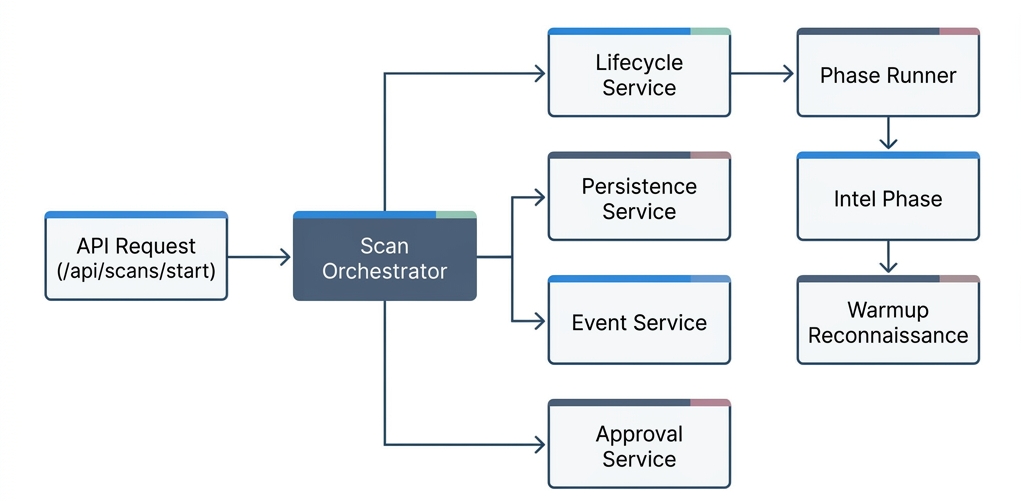
\includegraphics[width=0.75\textwidth]{langgraph_flow.png}
    \caption{Service-based scan flow demonstrating the progression of a run}
    \label{fig:langgraph_flow}
\end{figure}

Operationally, the runner service constructs worker callbacks for the recon lane,
opens analyzer context where needed, and emits structured scan events that are later
consumed by the SSE route. This implementation choice is particularly important from
an engineering standpoint: the frontend is never forced to poll opaque backend state.
Instead, it subscribes to a live stream of scan events that reflect the actual
runtime progression of the platform.

\subsection{Live Observability with Server-Sent Events}

One of the strongest implementation choices of the current project is the use of a
live event stream rather than ad hoc progress polling. The backend exposes
Server-Sent Events (SSE) for scan supervision, and the desktop UI subscribes to this
stream to update dashboards, statuses, approval banners, and activity panels in real
time.

This has two immediate benefits. The first is user experience: the pentester can see
the scan evolve without repeatedly refreshing the interface. The second is
traceability: the same events that feed the UI are persisted or cached as part of the
scan history, which makes later diagnosis easier when a run is interrupted or when a
report must explain the sequence of operations that produced a finding.

\subsection{Data Sanitization and Privacy Layer}

The privacy and safety strategy is implemented as a distributed concern rather than
as a single module. Several layers participate in reducing risk before data reaches
either a language model or an execution path.

\begin{enumerate}
    \item \textbf{API boundary protection:} the backend starts with explicit safety
    middleware that filters requests and centralizes rate-limiting behavior.
    \item \textbf{Prompt path protection:} the PrivacyGate node intercepts prompts,
    masks sensitive values, and restores them after the LLM response is received.
    \item \textbf{Execution path protection:} run-custom guardrails validate command
    families, target scope, and role compatibility before any action is executed.
    \item \textbf{Delivery protection:} report export and share-link flows support
    password-protected access so that generated outputs remain under operator control.
\end{enumerate}

An important practical result of this implementation is that the same security logic
appears in multiple places with different responsibilities: the API protects entry,
the sandbox protects execution, and the reporting path protects distribution.

\subsection{Analyzer, Findings, and Risk Enrichment}

The analyzer path embodies the practical classification engine of the platform. It
receives raw execution outputs, normalizes them through deterministic parsers, applies
the SSVC decision tree, and enriches verified findings with CVSS scores before
persisting structured analyzer reports.

This implementation is especially visible in two areas:
\begin{itemize}
    \item \textbf{Evidence enrichment:} verified findings are enriched with CVSS
    information and SSVC decisions before reaching the report generator.
    \item \textbf{Planner handoff:} analyzer results are aggregated and handed back
    into the planning path so that the next execution cycle is based on evidence
    rather than assumptions.
\end{itemize}

The architectural value of this implementation is therefore twofold: it transforms
tool outputs into durable knowledge, and it closes the loop between execution and
planning.

\subsection{RAG Pipeline and Chatbot Interface}

The retrieval path of the implemented project is organized around Qdrant and an Intel
resource model. The platform stores target-type-oriented resources, update
preferences, and project-level report and finding artifacts separately, which allows
retrieval to serve multiple contexts: planning, assistant interactions, and reporting.

On the user-facing side, the assistant path is integrated directly into the desktop
experience. The React frontend maintains the conversational state, while the backend
assistant route can access project memory, saved findings, and safe execution tools.
This turns the chatbot into a genuine operator aid rather than a detached natural
language layer.

\subsection{Desktop Workflows and Tauri Integration}

The desktop application implements the operator workflow that gives coherence to the
platform: project creation, target-type selection, scan launch, report review, client
delivery, and settings management. Because the UI is packaged with Tauri, the product
preserves the familiarity of a web interface while remaining distributed as a desktop
tool suitable for local use inside a controlled assessment environment.

\subsection{Report Generation and Client Delivery}

The reporting path is implemented as a durable backend task. When the operator
requests report generation, the backend creates a report run entry, invokes the
report generator, stores the Markdown report, derives the HTML representation, and
marks the task status as completed or failed.

The delivery path extends this logic. A dedicated share route can create or revoke a
client-facing link, optionally protect it with a password, and expose a scoped
viewer. On the export side, the report module packages protected downloads so that
the generated document does not circulate as an immediately open artifact.

\subsection{Target-Type-Aware Configuration}

One of the most distinctive implementation choices of PentaForge is the explicit
modeling of target types. The backend exposes a target-type catalog, dynamic field
extraction from Pydantic schemas, and editable information-gathering profiles. On
the frontend, the project creation dialog consumes this metadata to adapt the data
entry form to the selected target type, removing the common ambiguity found in
generic pentest tools that force every engagement into a single flat target field.

% ── Section 5 ─────────────────────────────────────────────────────────────
\section{Implementation of the Execution and Safety Path}

\subsection{Dedicated Sandbox Service}

Tool execution is isolated in a dedicated sandbox service exposed over HTTP inside
the Docker environment. The backend does not execute high-risk operational commands
directly in its own process. Instead, it delegates \texttt{run-custom} and
\texttt{run-python} style actions to the sandbox service, which validates the
request, reconstructs the execution context, and performs a second layer of scope
and policy checks.

This design has two major benefits. First, it sharply separates the control plane
from the execution plane. Second, it allows the sandbox image to contain the command
line tooling, wordlists, and execution environment needed by the agents without
inflating the trust placed in the main backend service.

\subsection{Command Guardrails and Resource Resolution}

The sandbox path is coupled with a guard module that classifies tools, detects
recon-role violations, validates network targets against the active scope, and
collects artifact paths created by a command. It also resolves shared resource paths
such as wordlists and SecLists entries into container-friendly locations.

In practice, this means that the implementation does not treat command execution as a
simple shell wrapper. It treats it as a policy-checked action with context, target,
role, and artifact semantics --- a critical property for a security product, because
the absence of such checks would make the platform itself a risk.

\subsection{Execution Context and Artifact Handling}

Beyond command validation, the execution lane preserves enough context for results to
remain useful after the tool finishes. The execution path transmits identifiers such
as project scope, target type, and role semantics together with the command request.
Generated outputs, logs, and evidence paths are then mapped back to project storage
and to the operator-facing reporting path, attributing each output to the right
project, the right scenario step, and the right downstream consumer.

\subsection{Desktop Integration Through Tauri}

On the frontend side, the Tauri shell provides a native desktop container around the
React application. The Tauri configuration defines the main window, the Vite
development workflow, and the production build coupling between the native shell and
the frontend bundle, offering the ergonomics of a modern web interface with lower
runtime weight than a full browser-engine desktop stack.

% ── Section 6 ─────────────────────────────────────────────────────────────
\section{End-to-End Execution on a Test Environment}

To validate the platform in realistic conditions, PentaForge was executed in its
containerized environment with the full operational path enabled: desktop UI,
backend API, Redis, Qdrant, and the isolated tool sandbox. The following scenario
illustrates how the implemented modules cooperate during a standard engagement.

\subsection{Phase 1: Engagement Setup and Project Initialization}

The workflow begins in the Projects page, where the operator creates an engagement,
selects the target type, and fills in the structured target information requested by
the schema for that type. Once the project is saved, the scan can be launched from
the dashboard. The backend immediately registers a runtime state, assigns a scan
identifier, and starts publishing SSE events such as \texttt{scan\_started},
\texttt{intel\_started}, and \texttt{intel\_completed}.

From the operator perspective, this first phase validates two things at once: the
data model is correctly instantiated, and the live observability path is functional.
The frontend does not need to infer progress heuristically; it displays what the
backend explicitly emits.

\begin{figure}[H]
    \centering
    % \includegraphics[width=0.85\textwidth]{ui_dashboard.png}
    \caption{PentaForge Operator Dashboard showing real-time target mapping}
    \label{fig:ui_dashboard}
\end{figure}

\subsection{Phase 2: Intel Preparation and Warmup Reconnaissance}

Once the scan begins, the runner service initializes the Intel node and then the
warmup recon workers. The Intel phase prepares the knowledge baseline of the
engagement, while the information-gathering and recon paths start building the first
usable memory of the target. Whenever a tool must be run remotely, the request is
sent to the sandbox service together with the active execution context.

At this point, the safety path becomes visible in the implementation. Commands are
validated for role and scope compatibility, and any required approval can be surfaced
back to the operator. The result is a supervised execution model: automation is used
to accelerate technical work, but not at the cost of losing operator control.

\subsection{Phase 3: Analysis, Enrichment, and Planning Feedback}

As tool results accumulate, the analyzer path consolidates them into structured
findings and summaries. These outputs are reused in multiple ways: they enrich memory
for later planning, they feed the report generator, and they populate the reporting
surfaces visible to the operator.

This phase is where the circular logic of the platform becomes clear. Each result is
interpreted, correlated with existing memory, and transformed into a planning input
for the next step, realizing a genuine feedback loop:
\emph{plan $\rightarrow$ execute $\rightarrow$ analyze $\rightarrow$ update memory
$\rightarrow$ plan again}. This loop is one of the core differentiators of
PentaForge compared with fragmented toolchains in which outputs remain disconnected.

\subsection{Phase 4: Reporting, Export, and Client Delivery}

When report generation is triggered, the backend stores a dedicated report task run,
creates the Markdown report, derives the HTML report, and makes both available in the
Reports page. From there, the operator can preview content, update the Markdown
version when necessary, generate a password-protected export package, or create a
share link for the client portal.

\begin{figure}[H]
    \centering
    % \includegraphics[width=0.85\textwidth]{ui_report_export.png}
    \caption{Generated finding detail showing evidence capture and SSVC decision}
    \label{fig:ui_report}
\end{figure}

% ── Section 7 ─────────────────────────────────────────────────────────────
\section{Validation, Evaluation, and Discussion}

\subsection{Introduction}

Validation is necessary to demonstrate that PentaForge satisfies its functional and
non-functional requirements. The platform combines several complex concerns: user
interaction, asynchronous scan orchestration, AI planning, sandboxed tool execution,
evidence classification, reporting, sharing, and protected downloads. The validation
approach therefore covers functional behavior, workflow continuity, security controls,
report quality, and user experience.

\subsection{Validation Strategy}

The validation strategy is based on five axes:

\begin{itemize}
    \item \textbf{Functional validation:} verifies that each main use case works as
    expected.
    \item \textbf{Workflow validation:} verifies that scan states, resume behavior,
    and scenario transitions are correct.
    \item \textbf{Security validation:} verifies scope enforcement, sandbox routing,
    download protection, and project data isolation.
    \item \textbf{Report validation:} verifies that the generated report is
    professional, complete, project-scoped, and free from invented vulnerabilities.
    \item \textbf{Usability validation:} verifies that the user can understand scan
    status, preview reports, and download deliverables without hidden steps.
\end{itemize}

\subsection{Functional Test Matrix}

\begin{longtable}{|p{0.08\textwidth}|p{0.24\textwidth}|p{0.28\textwidth}|p{0.30\textwidth}|}
\hline
\textbf{ID} & \textbf{Scenario} & \textbf{Expected result} & \textbf{Acceptance
criterion} \\
\hline
\endfirsthead
\hline
\textbf{ID} & \textbf{Scenario} & \textbf{Expected result} & \textbf{Acceptance
criterion} \\
\hline
\endhead
T01 & Create a web application project & Project appears in the projects list and
opens correctly. & Project metadata is persisted and target is displayed
consistently. \\
\hline
T02 & Start a scan on a valid target & Pipeline enters running state and emits live
updates. & UI shows planner, executer, analyzer, timer, and latest messages. \\
\hline
T03 & Generate checklist & Checklist is created from target type and project context.
& Checklist items are saved and remain available after refresh. \\
\hline
T04 & Generate plan after checklist & Plan is created from checklist items. &
Scenario identifiers are stable and visible in stored state. \\
\hline
T05 & Execute scenario & Tool request is routed through the sandbox. & Raw output,
exit code, and normalized result are stored. \\
\hline
T06 & Analyze evidence & Evidence is classified correctly. & Verified findings
require deterministic evidence, while noise remains informational or
inconclusive. \\
\hline
T07 & Stop and resume before checklist & Incomplete scan starts from scratch. & No
unstable partial data is reused as completed work. \\
\hline
T08 & Stop after checklist before plan & Plan is created on resume. & Checklist is
preserved and execution continues. \\
\hline
T09 & Stop during scenario execution & Running scenario restarts from executer. &
Completed scenarios are not repeated unless manually requested. \\
\hline
T10 & Regenerate report & Professional HTML preview is selected by default. & Report
cards show generated status and preview opens without requiring extra selection. \\
\hline
T11 & Download protected PDF & PDF download is password protected. & Opening the
downloaded file requires the configured password. \\
\hline
T12 & Download protected HTML package & HTML export is packaged and protected. & The
downloaded package behaves consistently with the pentester and client share
flows. \\
\hline
T13 & Delete project & All project data is removed. & Findings, history, reports,
share links, and project-scoped cache entries are deleted. \\
\hline
T14 & Generate report with no findings & Report states no verified findings. & It
includes methodology, coverage, limitations, and project history without invented
vulnerabilities. \\
\hline
T15 & Same target in two projects & Reports remain project-scoped. & Findings from
one project do not appear in another project unless generated there. \\
\hline
\caption{Functional test matrix}
\label{tab:functional_test_matrix}
\end{longtable}

\subsection{Workflow Validation}

Workflow validation focuses on the orchestration logic. A successful workflow must
also handle partial progress, operator interruptions, failed tools, inconclusive
evidence, and report regeneration.

\subsubsection{Checklist and Plan Validation}

\begin{longtable}{|p{0.22\textwidth}|p{0.30\textwidth}|p{0.38\textwidth}|}
\hline
\textbf{Artifact} & \textbf{Validation point} & \textbf{Reason} \\
\hline
\endfirsthead
\hline
\textbf{Artifact} & \textbf{Validation point} & \textbf{Reason} \\
\hline
\endhead
Checklist & Contains target-relevant items & Prevents generic or irrelevant scan
behavior. \\
\hline
Checklist & Saved before plan creation & Allows resume after interruption between
checklist and planning. \\
\hline
Plan & Uses stable scenario identifiers & Enables idempotent resume and accurate
progress tracking. \\
\hline
Plan & Marks scenario status explicitly & Allows completed, pending, running,
failed, and skipped states to be handled differently. \\
\hline
Plan & Links scenarios to evidence records & Allows report generation to explain
how a finding was produced. \\
\hline
\caption{Checklist and plan validation}
\label{tab:checklist_plan_validation}
\end{longtable}

\subsubsection{Analyzer Validation}

The analyzer must be conservative. A failed command, a missing tool, a model
suggestion, or a generic payload recommendation is not a verified vulnerability. The
analyzer validation criteria are:

\begin{itemize}
    \item A finding must reference an affected asset or endpoint.
    \item Evidence must come from the current project.
    \item Severity must match demonstrated impact.
    \item Inconclusive results must remain inconclusive.
    \item False positives must not appear in the risk table.
    \item Informational observations may appear in methodology or appendix sections,
    but not as verified vulnerabilities.
\end{itemize}

\subsection{Report Quality Validation}

\begin{longtable}{|p{0.24\textwidth}|p{0.30\textwidth}|p{0.36\textwidth}|}
\hline
\textbf{Quality criterion} & \textbf{Expected behavior} & \textbf{Validation
method} \\
\hline
\endfirsthead
\hline
\textbf{Quality criterion} & \textbf{Expected behavior} & \textbf{Validation
method} \\
\hline
\endhead
Executive clarity & The executive summary explains risk in business language. &
Review summary for concise risk, scope, and remediation urgency. \\
\hline
Finding completeness & Each finding includes severity, asset, description,
evidence, impact, and remediation. & Check all verified findings against the
report template. \\
\hline
Risk table format & The table lists each vulnerability, not only severity counts.
& Confirm columns: number, finding, severity, CVSS, confidence, status. \\
\hline
No hallucinated findings & The report does not invent vulnerabilities when none
were saved. & Compare report findings with project-scoped saved findings. \\
\hline
No internal noise & Client report does not expose agent debug traces or repetitive
tool errors. & Inspect report appendix and remove internal implementation
messages. \\
\hline
Download protection & Exported PDF and HTML packages are password protected. &
Open downloaded artifacts and confirm password prompt. \\
\hline
Default preview & Professional HTML is shown by default after regeneration. &
Regenerate report and confirm the preview panel opens the HTML report. \\
\hline
\caption{Report quality validation}
\label{tab:report_quality_validation}
\end{longtable}

\subsection{Security Control Validation}

\begin{longtable}{|p{0.20\textwidth}|p{0.30\textwidth}|p{0.40\textwidth}|}
\hline
\textbf{Control} & \textbf{Threat addressed} & \textbf{Validation expectation} \\
\hline
\endfirsthead
\hline
\textbf{Control} & \textbf{Threat addressed} & \textbf{Validation expectation} \\
\hline
\endhead
Scope validation & Tool execution outside authorized target & Commands targeting
out-of-scope hosts are rejected before sandbox execution. \\
\hline
Sandbox isolation & Local system compromise through tool execution & Tools run in
a controlled containerized environment with limited access. \\
\hline
Tool routing & Uncontrolled arbitrary command execution & Agent requests pass
through approved routing and policy checks. \\
\hline
Project isolation & Cross-project evidence leakage & Reports and findings load
only records associated with the current project. \\
\hline
Download protection & Unauthorized reading of exported report files & Exported PDF
and HTML artifacts require a password when opened. \\
\hline
Share token & Unauthorized report access & Client pages require a valid share token
and expose only report content, not internal scan state. \\
\hline
\caption{Security control validation}
\label{tab:security_control_validation}
\end{longtable}

\subsection{Performance and Scalability Discussion}

The performance of PentaForge depends on the interaction between the orchestrator,
the tool execution layer, the analyzer, and the storage layer. The design addresses
the most expensive operations through four mechanisms: target-type routing to avoid
irrelevant tools, result reuse to prevent repeated identical executions, evidence
summarization to reduce model input size, and SSE streaming to keep the UI responsive
during long-running tasks.

\begin{longtable}{|p{0.24\textwidth}|p{0.32\textwidth}|p{0.34\textwidth}|}
\hline
\textbf{Bottleneck} & \textbf{Effect} & \textbf{Optimization} \\
\hline
\endfirsthead
\hline
\textbf{Bottleneck} & \textbf{Effect} & \textbf{Optimization} \\
\hline
\endhead
Repeated commands & Increased scan duration and duplicate target traffic & Use
project-scoped command cache. \\
\hline
Large raw outputs & Slow analyzer and report prompts & Store raw evidence but pass
normalized snippets to reasoning steps. \\
\hline
Long-running scans & UI appears blocked if progress is not streamed & Use
server-sent events and persistent progress state. \\
\hline
Tool installation gaps & Failed scenarios and noisy logs & Maintain sandbox image
and tool inventory checks. \\
\hline
Report regeneration & User waits for formatting and export tasks & Save report
artifacts and regenerate only when requested. \\
\hline
\caption{Performance bottlenecks and optimizations}
\label{tab:performance_bottlenecks}
\end{longtable}

\subsection{Limitations}

\begin{itemize}
    \item Some security tools may be absent from the sandbox image or may produce
    unstructured output that is difficult to parse.
    \item Some target types require authenticated credentials to reach meaningful
    attack surfaces.
    \item Fully autonomous exploitation must remain constrained by scope and safety
    policies.
    \item Report generation quality depends on the quality of saved evidence.
    \item Resume behavior requires strict state discipline; any missing checkpoint
    can lead to conservative restarts.
    \item PDF generation and password protection must be tested on the same platform
    used for delivery because browser preview behavior can differ from downloaded
    file behavior.
\end{itemize}

\subsection{Future Improvements}

\begin{itemize}
    \item Add a visual state inspector for scan checkpoints and scenario status.
    \item Implement a dedicated tool-result cache dashboard for repeated commands.
    \item Add stronger authenticated testing workflows with secure credential
    storage.
    \item Add role-based access control for multi-user deployments.
    \item Improve report customization with templates for executive, technical, and
    remediation-focused audiences.
    \item Add more deterministic parsers for common tools to reduce model dependency.
    \item Add automated retest workflows that compare old evidence with fresh
    remediation checks.
\end{itemize}

\section{Conclusion}

This chapter demonstrated the concrete realization of PentaForge as a working
platform. The sprint-by-sprint narrative showed how the platform grew incrementally
from a persistence foundation in Sprint 1 to a fully packaged and hardened product
in Sprint 6, with each iteration delivering a testable increment that built directly
on the previous one. The architecture described in Chapter 3 was translated into a
desktop application, a FastAPI backend, dedicated scan services, a sandboxed
execution lane, specialized storage components, and a complete reporting and delivery
path. Beyond the individual modules, the implementation validated a broader design
principle: automation becomes valuable when it is coupled with clear boundaries,
explicit operator control, and durable project state.

By grounding the implementation in real route handlers, service layers, target-type
metadata, SSE observability, report generation, and share-link delivery, the project
demonstrates that PentaForge is not merely a conceptual multi-agent system. It is a
coherent operational platform whose components already interact in a structured and
extensible manner.

% ── Restore default page style ─────────────────────────────────────────────
\pagestyle{fancy}

% ==================== GENERAL CONCLUSION ====================
\newpage
\thispagestyle{fancy}
\chapter*{General Conclusion}
\addcontentsline{toc}{chapter}{General Conclusion}

The constant evolution of cyber threats, coupled with the exponential growth of organizational 
attack surfaces, has highlighted the structural limitations of traditional, manual 
penetration testing. Organizations require security assessments that are scalable, 
frequent, and highly accurate, without compromising on depth or methodological rigor.

This end-of-studies project, conducted within the cybersecurity team at Talan, aimed to 
solve these challenges through the design and implementation of \textbf{PentaForge}: an 
open-source, AI-powered automated penetration testing platform. 

Throughout this project, we successfully translated complex theoretical concepts into a 
fully functional product. We designed a \textbf{multi-agent architecture} capable of 
orchestrating specialized AI agents (Recon, Exploit, Verify, Report, Retest) to autonomously 
navigate the entire penetration testing lifecycle. We integrated an \textbf{SSVC decision engine} 
to replace static vulnerability scoring with context-aware prioritization. Furthermore, 
we built a persistent \textbf{RAG-powered conversational interface} that bridges the gap 
between raw technical outputs and executive understanding, all while strictly guaranteeing 
the confidentiality of target data through an automated sanitization layer.

From a technical standpoint, this internship was profoundly enriching. It provided an
opportunity to deepen skills in LLM-assisted application design, backend
orchestration with FastAPI and dedicated service layers, and desktop interface
engineering using React and Tauri. The adoption of the Scrum methodology fostered a
professional approach to iterative development, continuous integration, and
stakeholder feedback.

While PentaForge currently represents a powerful enhancement to the pentester's toolkit, 
several perspectives can be explored to expand its capabilities:
\begin{itemize}
    \item \textbf{Integration into CI/CD Pipelines (DevSecOps):} Allowing PentaForge to 
    automatically spawn lightweight agent clusters to test new infrastructure builds 
    before they are merged into production.
    \item \textbf{Continuous Security Validation:} Transitioning from point-in-time scans 
    to a continuous red-teaming mode, where agents persistently monitor the attack surface 
    and react to new CVEs published by the Intel feed in real time.
    \item \textbf{Advanced Privilege Escalation Models:} Enhancing the Exploit Agent
    with richer graph-oriented reasoning and privilege-correlation models to
    autonomously discover complex Active Directory misconfigurations and cross-cloud
    IAM privilege chains.
\end{itemize}

Ultimately, PentaForge demonstrates that artificial intelligence is not meant to replace 
human security experts, nor to independently perform the full work of a penetration 
tester from end to end. Its value lies in serving as a force multiplier: helping 
analysts preserve context, accelerate repetitive operations, and identify potential 
vulnerabilities that must still be interpreted, validated, and prioritized by a human 
professional. By automating the mundane and accelerating the complex, it allows security 
professionals to focus on what truly matters: creative analysis, strategic remediation, 
and staying one step ahead of the adversary.

% ==================== BIBLIOGRAPHY ====================
\cleardoublepage
\addcontentsline{toc}{chapter}{Bibliography}
\begin{thebibliography}{99}

\bibitem{triaxiomTimeline}
Triaxiom Security, \textit{What is the Typical Timeline for a Penetration Test?}, \url{https://www.triaxiomsecurity.com/blog/typical-timeline-for-a-penetration-test/} (accessed 2026).

\bibitem{valuementorLifecycle}
ValueMentor, \textit{Penetration Testing Service Lifecycle}, \url{https://valuementor.com/blogs/penetration-testing-service-inside-the-complete-assessment-lifecycle} (accessed 2026).

\bibitem{autosecagent2026}
AutoSecAgent, \textit{The Journal of Supercomputing} (Springer Nature), 2026, \url{https://link.springer.com/article/10.1007/s11227-026-08439-z}.

\bibitem{emazzantiTools}
eMazzanti Technologies, \textit{Benefits and Limitations of Automated Tools in Penetration Testing}, \url{https://www.emazzanti.net/benefits-and-limitations-of-automated-tools-in-penetration-testing/} (accessed 2026).

\bibitem{pentestgpt2023}
PentestGPT, arXiv:2308.06782, \url{https://arxiv.org/pdf/2308.06782} (accessed 2026).

\bibitem{hedgehogRetesting}
Hedgehog Security, \textit{Remediation Validation and Retesting}, \url{https://www.hedgehogsecurity.co.uk/blog/remediation-validation-retesting-close-the-loop} (accessed 2026).

\bibitem{redleggRetesting}
RedLegg, \textit{The Role of Retesting in Vulnerability Remediation Validation}, \url{https://www.redlegg.com/blog/vulnerability-remediation-retesting-guide} (accessed 2026).

\bibitem{halockVerification}
HALOCK, \textit{Remediation Verification}, \url{https://www.halock.com/penetration-testing/remediation-verification/} (accessed 2026).

\bibitem{cycognitoPentest}
CyCognito, \textit{Penetration Testing} ("Penetration Testing in 2025"), \url{https://www.cycognito.com/learn/penetration-testing/} (accessed 2026).
\bibitem{ptes}
PTES Technical Guidelines, \textit{Penetration Testing Execution Standard},
\url{http://www.pentest-standard.org/index.php/Main_Page} (accessed 2026).
\bibitem{mitreattack}
MITRE Corporation, \textit{MITRE ATT\&CK Framework},
\url{https://attack.mitre.org} (accessed 2026).
\bibitem{threatexploitFP}
ThreatExploit AI, \textit{The Hidden Cost of False Positives: Why Scanners Alone
Aren't Enough}, \url{https://threatexploit.ai/en/blog/false-positives-scanners-vs-pentesting}
(accessed 2026).
\bibitem{bishopfoxAI}
Bishop Fox, \textit{AI Tooling Impact on Penetration Testing Engagements},
cited in RedFox Security, The State of AI Pentesting in 2026,
\url{https://www.redfoxsec.com/blog/the-state-of-ai-pentesting-in-2026-trends-statistics-and-whats-next}
(accessed 2026).

\bibitem{brightdefense2026}
Bright Defense, \textit{120+ Penetration Testing Statistics for 2026},
\url{https://www.brightdefense.com/resources/penetration-testing-statistics}
(accessed 2026).
\bibitem{pentestgpt2023}
G. Deng et al., \textit{PentestGPT: Evaluating and Harnessing Large Language
Models for Automated Penetration Testing}, arXiv:2308.06782,
\url{https://arxiv.org/pdf/2308.06782} (accessed 2026).

\bibitem{burpsuiteAI}
PortSwigger, \textit{Burp Suite AI --- Explore Issue and AI-Assisted Testing},
\url{https://portswigger.net/burp/documentation/desktop/ai-features}
(accessed 2026).

\bibitem{kaligpt}
KaliGPT, \textit{KaliGPT --- AI-Assisted Penetration Testing on Kali Linux},
\url{https://github.com/markusvalk/kaligpt} (accessed 2026).

\bibitem{nodezero}
Horizon3.ai, \textit{NodeZero --- Autonomous Penetration Testing Platform},
\url{https://www.horizon3.ai/nodezero} (accessed 2026).

\bibitem{shannon}
Keygraph, \textit{Shannon --- Open-Source White-Box AI Pentester},
\url{https://github.com/keygraph/shannon} (accessed 2026).
\bibitem{qwen25report}
Qwen Team, \textit{Qwen2.5 Technical Report}, arXiv:2412.15115,
\url{https://arxiv.org/abs/2412.15115} (2024).
\bibitem{geminiRateLimits}
Google, \textit{Gemini API Rate Limits --- Usage Tiers and Quotas},
\url{https://ai.google.dev/gemini-api/docs/rate-limits} (accessed 2026).

\bibitem{llmstatsFlash}
LLM Stats, \textit{Gemini 2.5 Flash vs.\ Gemini 2.5 Pro --- Benchmark Comparison},
\url{https://llm-stats.com/models/compare/gemini-2.5-flash-vs-gemini-2.5-pro}
(accessed 2026). Global MMLU-Lite score for Gemini 2.5 Flash: 88.4\%.

\bibitem{mistralDocs}
Mistral AI, \textit{Rate Limits and Usage Tiers},
\url{https://docs.mistral.ai/admin/user-management-finops/tier} (accessed 2026).
\end{thebibliography}

\end{document}
